% \chapter{Experiment}
\chapter{\chapterFive}
\label{chp:5}

\textit{After describing our proposed system as an attempt to achieve this thesis' goals in the previous chapter, this chapter continues with an explanation of several experiment setups and results. This chapter starts by a presentation on two chosen SRAMs that used in experiments; Microchip 23LC1024 and Cypress CY62256NLL. Afterwards, the testing results on two bit selection algorithms (neighbor analysis and data remanence approach) and the stable bits produced by these algorithms are displayed. The chapter continues with examination on our proposed PUF challenge and a presentation on our complete enrollment scheme. Next, testing on the designed secure data protection and key storage scheme is shown. Experiment outcomes on storing bitcoin private key will conclude this chapter.}

\section{Chosen Off-The-Shelf SRAMs}
The first step to do in this thesis implementation is looking for off-the-shelf SRAM components to be the root-of-trust in our SRAM PUF project.
Due to numerous SRAM types available in the market, we need to define several requirements for the SRAM first. The main requirements on the SRAM are easy to get (a simple google search should show some e-commerce websites to buy from), can be bought in small quantity ($\leq$ 5 pieces), stand-alone component (available without buying extra component, e.g. not embedded in an FPGA), inexpensive (cost less than \euro{}5), reasonable memory size ($\geq$ 64kb). These criteria are chosen due to some product only sold to a company or an entity that willing to buy in a big quantity or has to be custom made. There are two SRAM types purchased and tested here; Microchip 23LC1024 and Cypress CY62256NLL.

% As mentioned in Chapter 2, to be qualified as a PUF candidate, an SRAM has to be stable in various conditions. This means if it is given various power input or used in varied temperatures or utilized for a long time, the initialized SRAM values has to remain similar or only has little changes. Under any condition, there should be no overlap between HD\textsubscript{intra} and HD\textsubscript{inter}. Moreover, the SRAM has to have a sufficient amount of randomness, shown by having equal distributions between 1's 0's on its values.  To ensure the quality of these two SRAMs, there are several experiments performed on each SRAM, such as calculating HD\textsubscript{intra} and HD\textsubscript{inter} given the whole memory value as the challenge and also the distribution of 1's and 0's inside SRAM memory.
%
\subsubsection{Microchip 23LC1024}
The Microchip Technology Inc. 23A1024/23LC1024 is a 1024 Kbit Serial SRAM device. This SRAM is very popular, shown by many references available online and several GitHub repositories intended just to access this SRAM. The reason of its popularity can be traced to its cheap price, small size, and easy-to-use. The price is ranging from \euro{}1.5-3.5. This device has eight pins which contribute significantly to its small footprint (it has dimension of 9.271 x 6.35 x 3.302 mm).
It is easy to use because it provides SPI connection which simplified the communication, and has three modes available; SPI (Serial Peripheral Interface), SDI (Serial Dual Interface) and SQI (Serial Quad Interface). Its voltage range also quite large, ranging from 2.5-5.5V. Figure \ref{fig:23LC1024} shows the Microchip 23LC1024.

\begin{figure}[tph!]
    \centerline{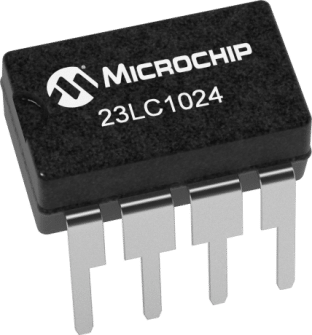
\includegraphics[width={0.2\textwidth}]{images/23lc1024}}
    \caption{SRAM Microchip 23LC1024 \cite{23lc1024}.}
    \label{fig:23LC1024}
\end{figure}

% There are ten SRAMs Microchip 23LC1024 that were available during the experiment. To check whether this SRAM is a justifiable candidate for PUF, several testings are performed.
% First, the number of 1's and 0's in memory after a start is calculated. Unfortunately, the average distribution of 1's and 0's are not similar, 1's occupy 70\% and 0's fill the remaining 30\%.
% Second, HD\textsubscript{intra} and HD\textsubscript{inter} are calculated on these chips. The calculation is done using twenty data of chip memory values on each chip which retrieved at room temperature, 5V input and 10 seconds interval between retrieval attempts. From these chips, the average HD\textsubscript{intra} is 6.18\% and the average HD\textsubscript{inter} is 42.54\%.
% Third, the effect of voltage variation on the HD\textsubscript{intra} and HD\textsubscript{inter} are also evaluated. The calculation is done using memory values on each chip which retrieved on room temperature and 10 seconds interval between retrieval attempts. The voltage range is between 2.5V and 5V with 0.5V increase on a step. On each step, there are three data retrieved. Using these data, voltage variation results in an average HD\textsubscript{intra} 8.21\% and an average HD\textsubscript{inter} 42.59\%.
%
% \begin{figure}[tph!]
%     \centerline{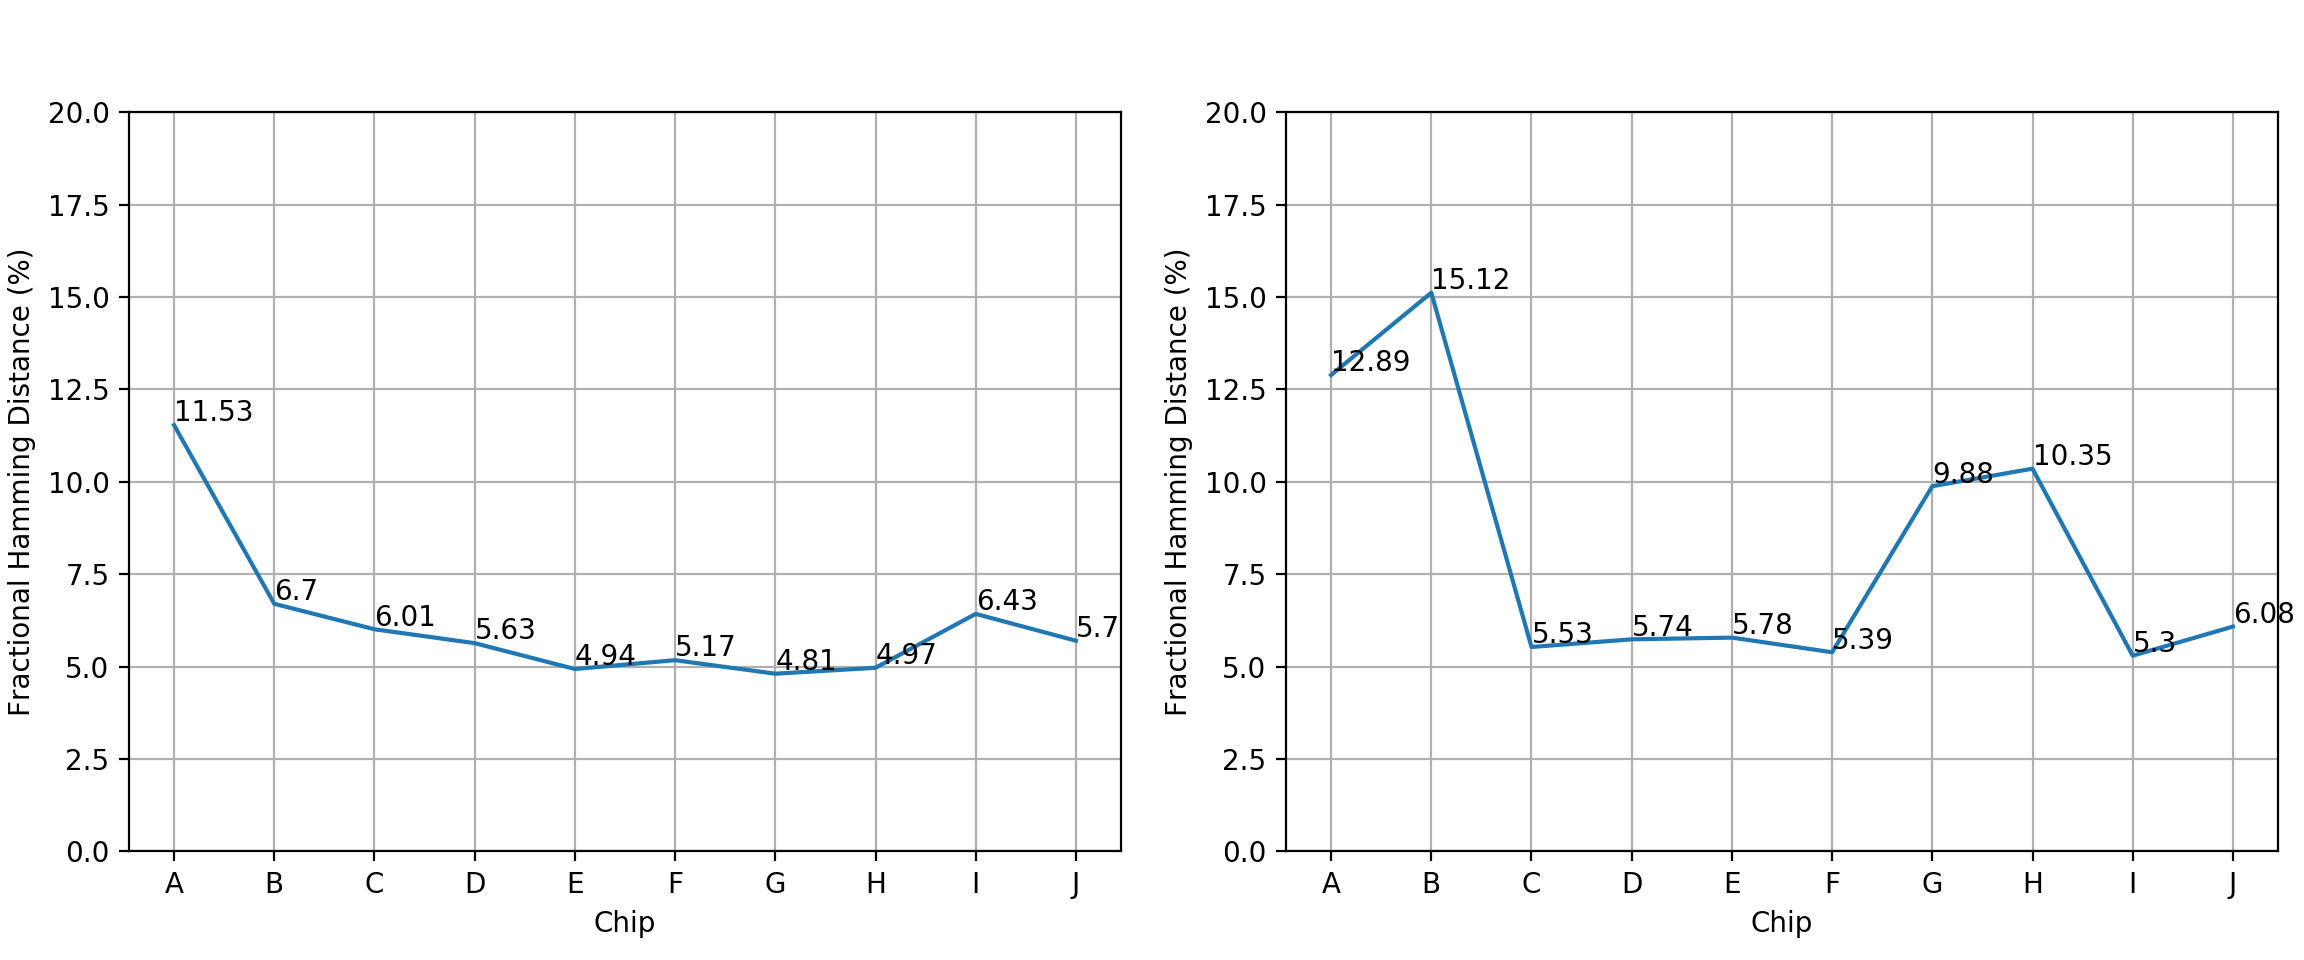
\includegraphics[width={\textwidth}]{images/23lc1024_hd_intra}}
%     \caption{HD\textsubscript{intra} of ten SRAMs Microchip 23LC1024. The left is HD\textsubscript{intra} with constant voltage, the right one is tested based on the voltage variation.}
%     \label{fig:23lc1024_hd_intra}
% \end{figure}
%
% Based on these experiments, SRAM Microchip 23LC1024 shows questionable results. First, the distribution of 1's and 0's inside the SRAM is not balanced. Second, a voltage variation shows that it significantly affects the  HD\textsubscript{intra}. Fortunately, there is no overlap between HD\textsubscript{intra} and HD\textsubscript{inter}. Even though these outcomes make us doubtful on this SRAM quality as an SRAM PUF candidate, we decided to continue using this SRAM in further experiments. Hopefully, when we locate the stable bits inside the SRAM, the experiments done on the stable bits will show a better result than this result.

\subsubsection{Cypress CY62256NLL}
The Cypress CY62256NLL is a 256k bit SRAM device. Even though this device is less popular than Microchip 23LC1024, it's still widely used. One of the reason is that this device has an automatic power-down feature, reducing the power consumption by 99.9 percent when deselected. Unlike Microchip 23LC1024, Cypress CY62256NLL doesn't have an SPI connection which complicates the communication. To communicate, one should utilize its twenty-eight pins available. Since it has many pins, this contributes to its significantly larger size compared to Microchip 23LC1024. Specifically, its size is 37.592 × 13.97 × 4.953 mm and produced using 90nm technology. Its voltage range is ranging from 4.5V-5.5V. Figure \ref{fig:CY62256NLL} shows Cypress CY62256NLL.

\begin{figure}[tph!]
    \centerline{
\includegraphics[width={0.4\textwidth}]{images/cy62256nll}}
    \caption{SRAM Cypress CY62256NLL \cite{CY62256NLL}.}
    \label{fig:CY62256NLL}
\end{figure}

% There are five Cypress CY62256NLL SRAMs that were available during experiment. Similar like on previous SRAM, several testing are performed to check whether this SRAM is a justifiable candidate for PUF.
% First, the number of 1's and 0's in an initialization is counted. Fortunately, unlike the 23LC1024, the average distribution of 1's and 0's are similar, both occupy 50\% of total bits available.
% Next,
% HD\textsubscript{intra} and HD\textsubscript{inter} are calculated on both chips. The calculation is done using twenty data of chip memory values on each chip which retrieved at room temperature, 5V input and 10 seconds interval between retrieval attempts.
% From these chips, the average HD\textsubscript{intra} is 4.85\% and the average HD\textsubscript{inter} is 39.28\%.
% Last, the effect of voltage variation on the HD\textsubscript{intra} and HD\textsubscript{inter} are also evaluated. The calculation is done using chip memory values on each chip which retrieved on room temperature and 10 seconds interval between retrieval attempts. The voltage range is between 4.5V and 5V with 0.1V increase on each step. On each step, there are ten data enrolled.
% The average HD\textsubscript{inter} on voltage variation is 38.59\%, while HD\textsubscript{intra} is 3.58\%. Figure \ref{fig:cy62256nll_hd_intra} shows the HD\textsubscript{intra} between the constant and the variated voltage.
%
% \begin{figure}[tph!]
%     \centerline{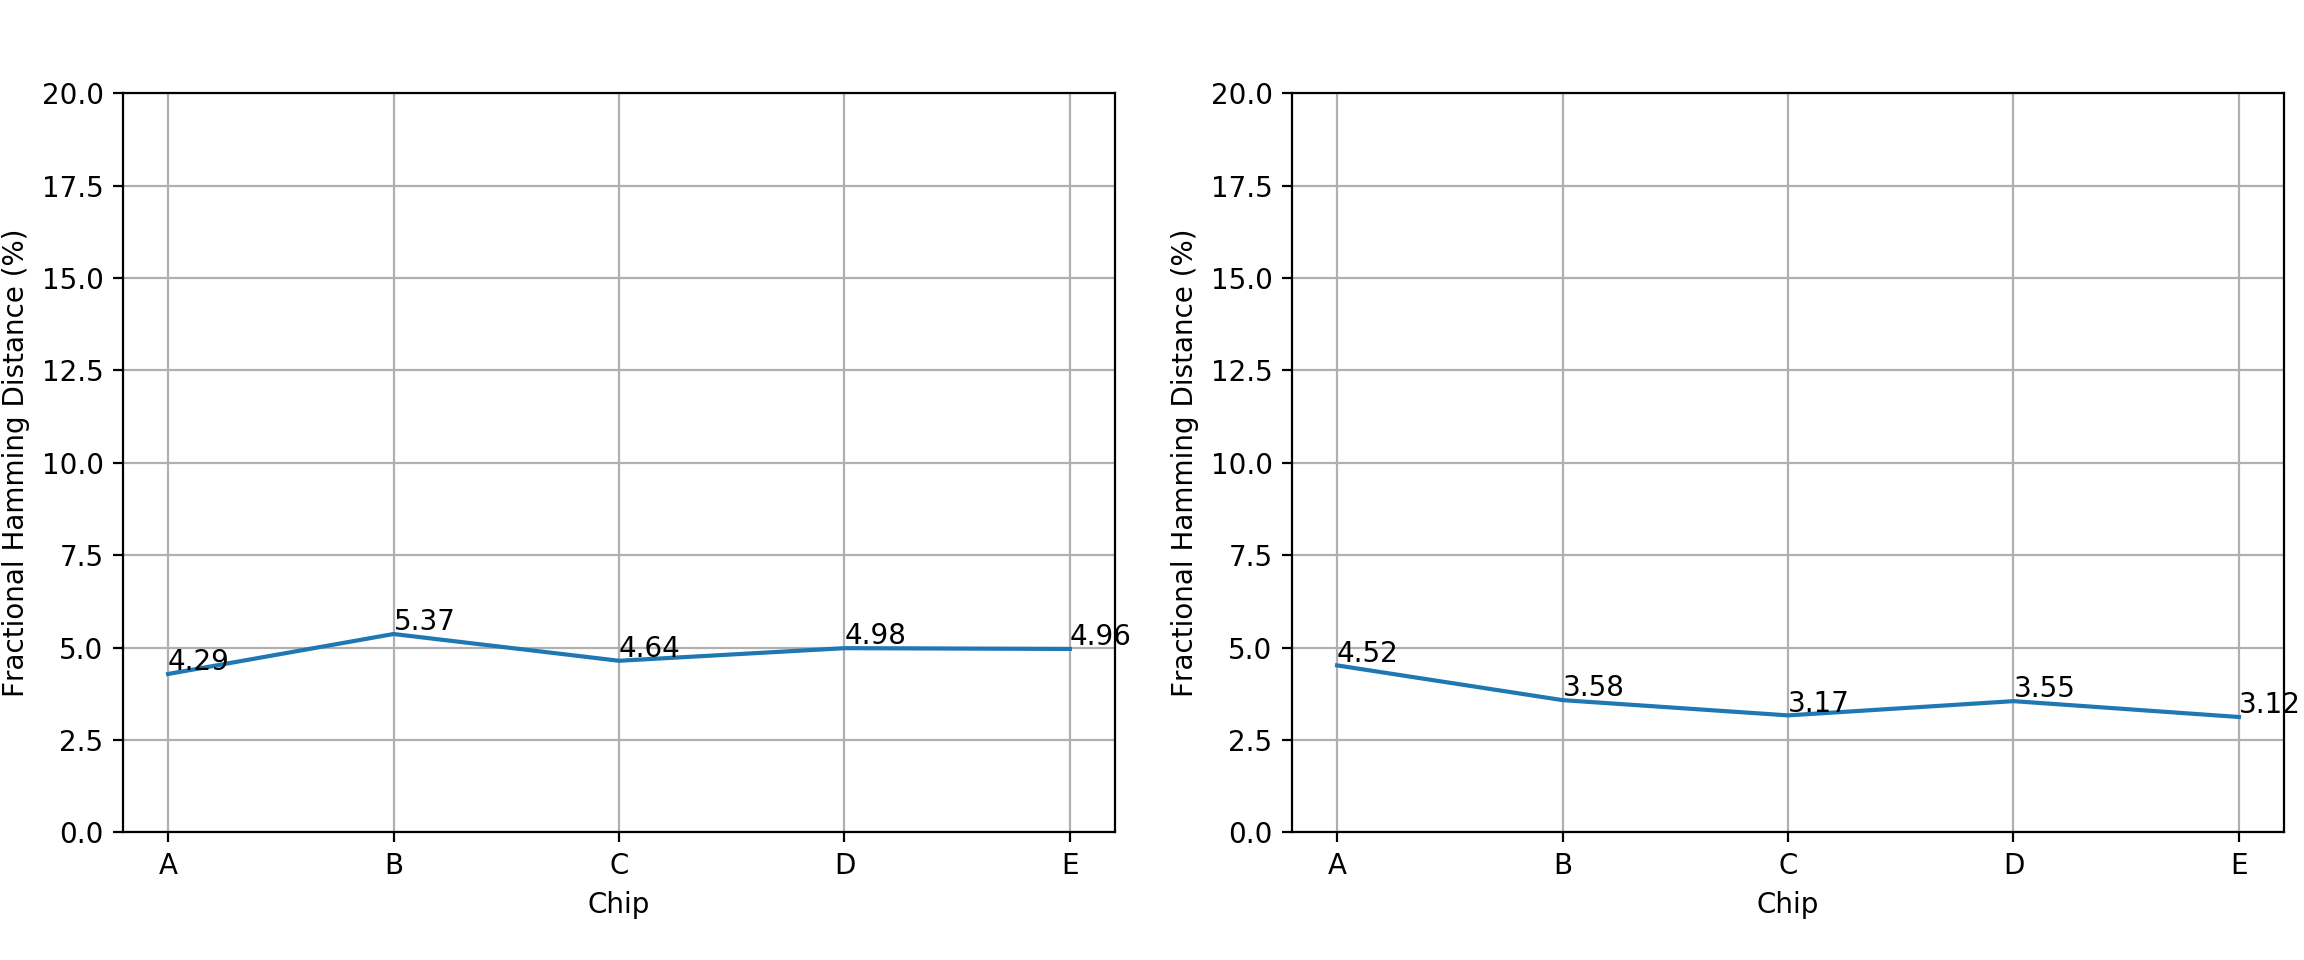
\includegraphics[width={\textwidth}]{images/cy62256nll_hd_intra}}
%     \caption{HD\textsubscript{intra} of five SRAMs Cypress CY62256NLL. The left is HD\textsubscript{intra} with constant voltage, the right one is tested based on the voltage variation.}
%     \label{fig:cy62256nll_hd_intra}
% \end{figure}
%
% The results shown above indicate that SRAM Cypress CY62256NLL is a qualified candidate for SRAM PUF. A well distributed 0's and 1's inside SRAM memory, voltage variation has little effect on HD\textsubscript{intra} and HD\textsubscript{inter}, and no overlap between HD\textsubscript{intra} and HD\textsubscript{inter} lead us to continue using this SRAM on further experiments.

\section{Automated PUF Profiling System}
To increase the experiment's efficiency, an automated PUF profiling system is constructed. The system consists of a PC, act as a master, and an Arduino connected to an external SRAM component which acts as a slave. A custom protocol was designed to communicate between them. It is specifically designed to be generic and usable for all types of PUF profiling measurements. The software on Arduino side waits for measurement commands sent by PC on the serial link after booting. The designed protocol is dedicated for read bytes, write bytes, and SRAM disable/enable. The system also supported parallel profiling which significantly increases the effectivity. Figure \ref{fig:puf_profiling} shows the setup and the schematic to profile four SRAMs Cypress CY62256NLL concurrently using four Arduino.

\begin{figure}[tph!]
    \centerline{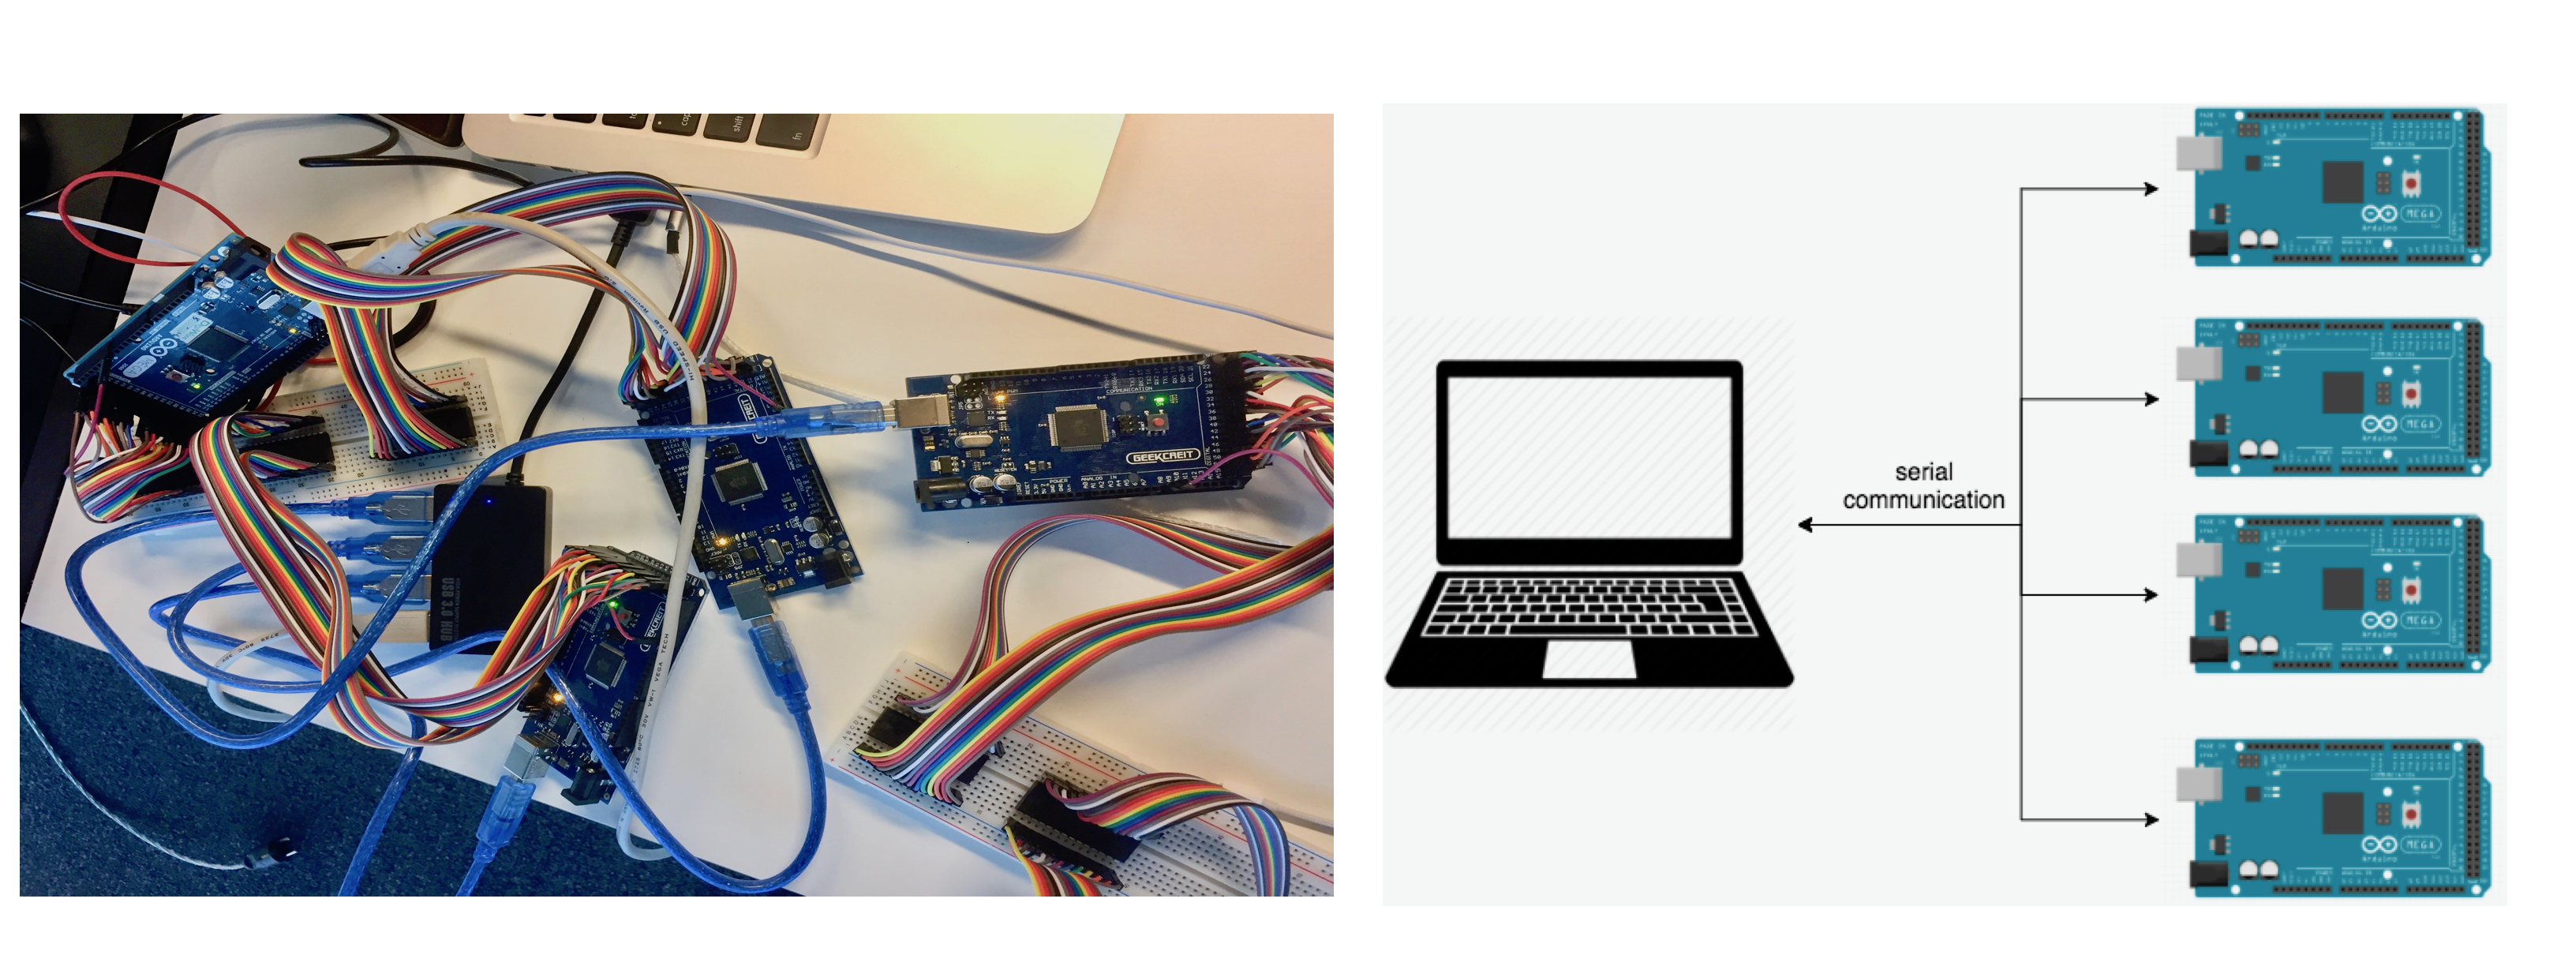
\includegraphics[width={\textwidth}]{images/setup}}
    \caption{Automated PUF profiling setup using a PC and four Arduino. Left picture shows the actual setup, while the right picture displays the schematic of such setup.}
    \label{fig:puf_profiling}
\end{figure}

\section{Testing on Chosen Off-The-Shelf SRAMs}

As mentioned in Chapter 2, to be qualified as a PUF candidate, an SRAM has to be stable in various conditions. This means if it is given various power input or used in varied temperatures or utilized for a long time, the initialized SRAM values has to remain similar or only has little changes. Under any condition, there should be no overlap between HD\textsubscript{intra} and HD\textsubscript{inter}. Moreover, the SRAM has to have a sufficient amount of randomness, shown by having equal distributions between 1's 0's on its values.  To ensure the quality of these two SRAMs, there are several experiments performed on each SRAM, such as calculating HD\textsubscript{intra} and HD\textsubscript{inter} given the whole memory value as the challenge and also the distribution of 1's and 0's inside SRAM memory.

\subsubsection{Microchip 23LC1024}
There are ten SRAMs Microchip 23LC1024 that were available during the experiment. To check whether this SRAM is a justifiable candidate for PUF, several testings are performed.
First, the number of 1's and 0's in memory after a start is calculated. Unfortunately, the average distribution of 1's and 0's are not similar, 1's occupy 70\% and 0's fill the remaining 30\%.
Second, HD\textsubscript{intra} and HD\textsubscript{inter} are calculated on these chips. The calculation is done using twenty data of chip memory values on each chip which retrieved at room temperature, 5V input and 10 seconds interval between retrieval attempts. From these chips, the average HD\textsubscript{intra} is 6.18\% and the average HD\textsubscript{inter} is 42.54\%.
Third, the effect of voltage variation on the HD\textsubscript{intra} and HD\textsubscript{inter} are also evaluated. The calculation is done using memory values on each chip which retrieved on room temperature and 10 seconds interval between retrieval attempts. The voltage range is between 2.5V and 5V with 0.5V increase on a step. On each step, there are three data retrieved. Using these data, voltage variation results in an average HD\textsubscript{intra} 8.21\% and an average HD\textsubscript{inter} 42.59\%.

\begin{figure}[tph!]
    \centerline{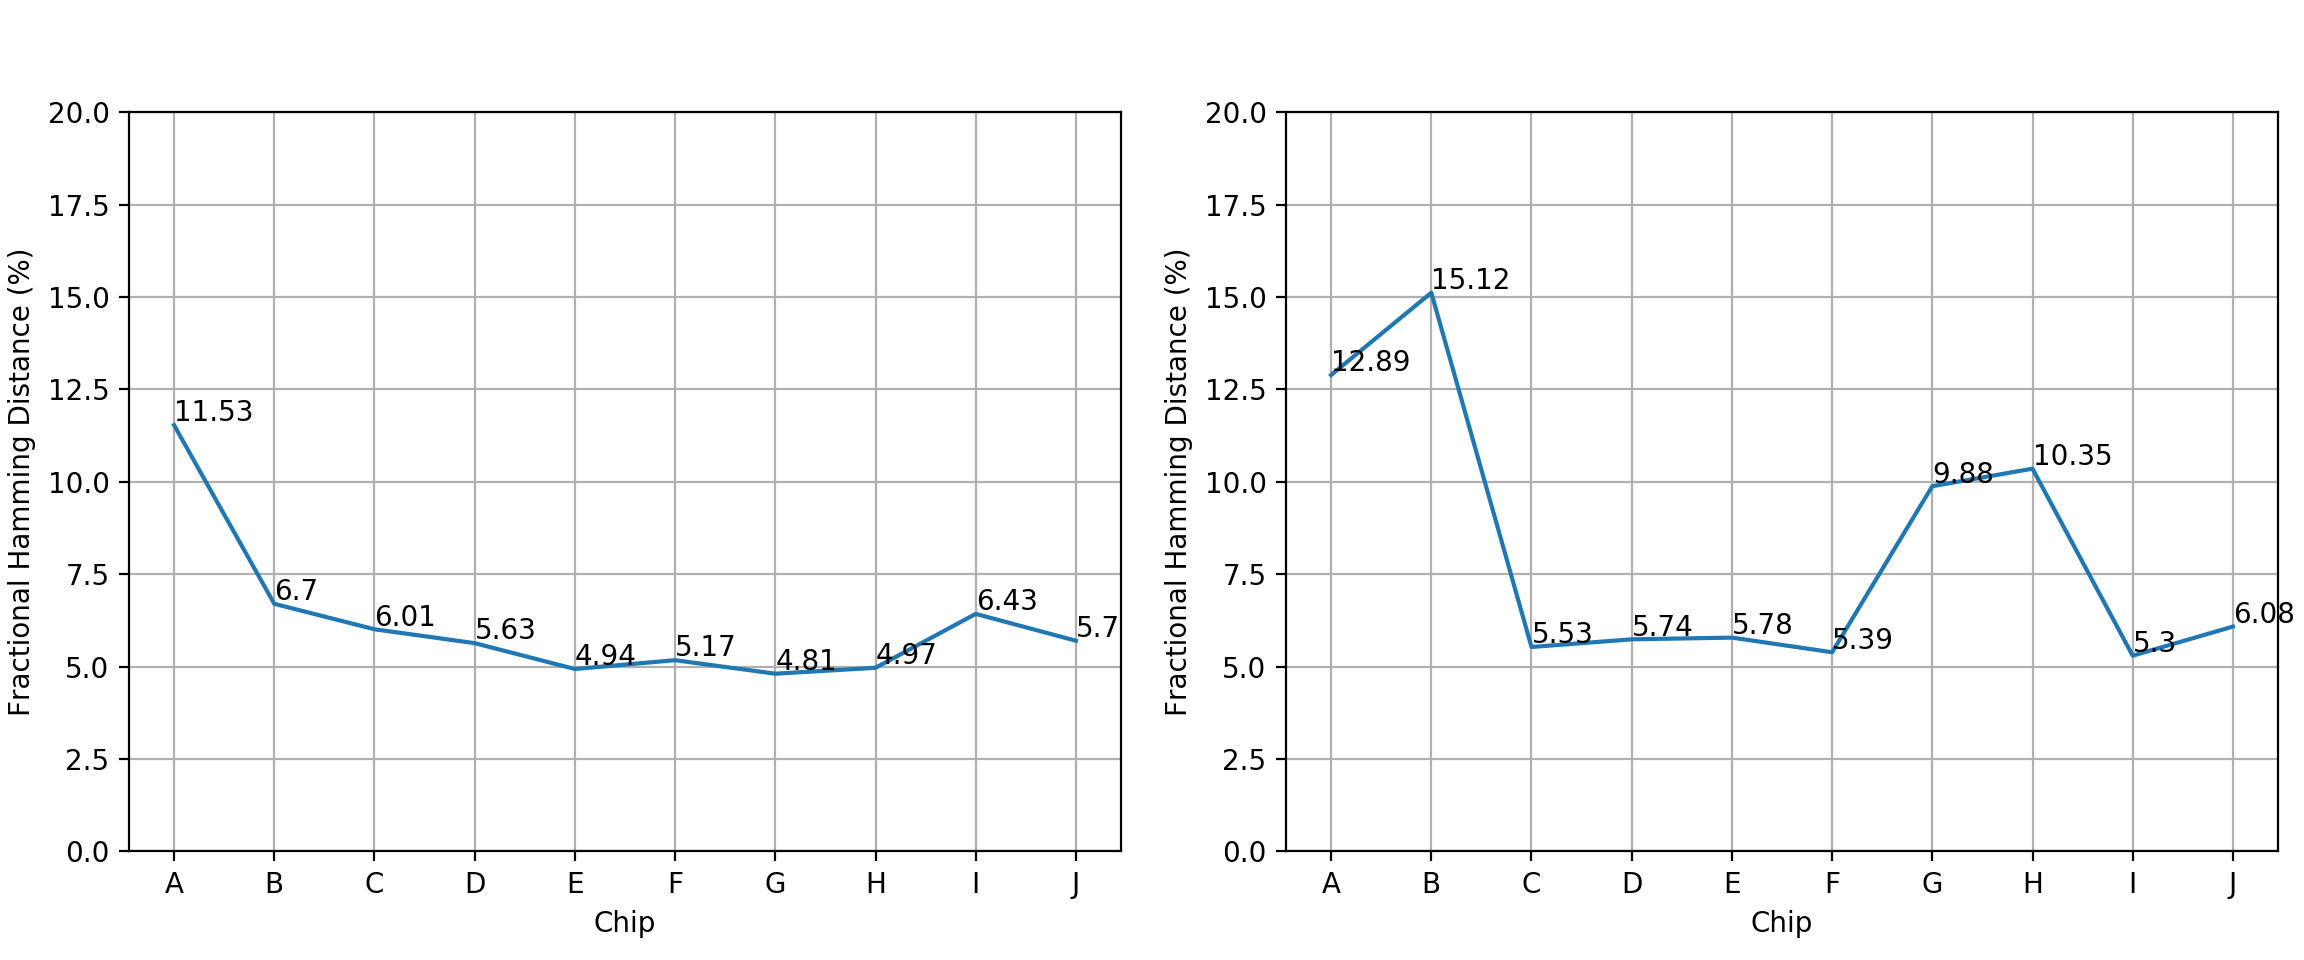
\includegraphics[width={\textwidth}]{images/23lc1024_hd_intra}}
    \caption{HD\textsubscript{intra} of ten SRAMs Microchip 23LC1024. The left figure is the testing result of HD\textsubscript{intra} with constant voltage, the right one is tested based on the voltage variation.}
    \label{fig:23lc1024_hd_intra}
\end{figure}

Based on these experiments, SRAM Microchip 23LC1024 shows questionable results. First, the distribution of 1's and 0's inside the SRAM is not balanced. Second, a voltage variation shows that it significantly affects the  HD\textsubscript{intra}. Fortunately, there is no overlap between HD\textsubscript{intra} and HD\textsubscript{inter}. Even though these outcomes make us doubtful on this SRAM quality as an SRAM PUF candidate, we decided to continue using this SRAM in further experiments. Hopefully, when we locate the stable bits inside the SRAM, the experiments done on the stable bits will show a better result than this result.

\subsubsection{Cypress CY62256NLL}

There are five Cypress CY62256NLL SRAMs that were available during experiment. Similar like on previous SRAM, several testing are performed to check whether this SRAM is a justifiable candidate for PUF.
First, the number of 1's and 0's in an initialization is counted. Fortunately, unlike the 23LC1024, the average distribution of 1's and 0's are similar, both occupy 50\% of total bits available.
Next,
HD\textsubscript{intra} and HD\textsubscript{inter} are calculated on both chips. The calculation is done using twenty data of chip memory values on each chip which retrieved at room temperature, 5V input and 10 seconds interval between retrieval attempts.
From these chips, the average HD\textsubscript{intra} is 4.85\% and the average HD\textsubscript{inter} is 39.28\%.
Last, the effect of voltage variation on the HD\textsubscript{intra} and HD\textsubscript{inter} are also evaluated. The calculation is done using chip memory values on each chip which retrieved on room temperature and 10 seconds interval between retrieval attempts. The voltage range is between 4.5V and 5V with 0.1V increase on each step. On each step, there are ten data enrolled.
The average HD\textsubscript{inter} on voltage variation is 38.59\%, while HD\textsubscript{intra} is 3.58\%. Figure \ref{fig:cy62256nll_hd_intra} shows the HD\textsubscript{intra} between the constant and the variated voltage.

\begin{figure}[tph!]
    \centerline{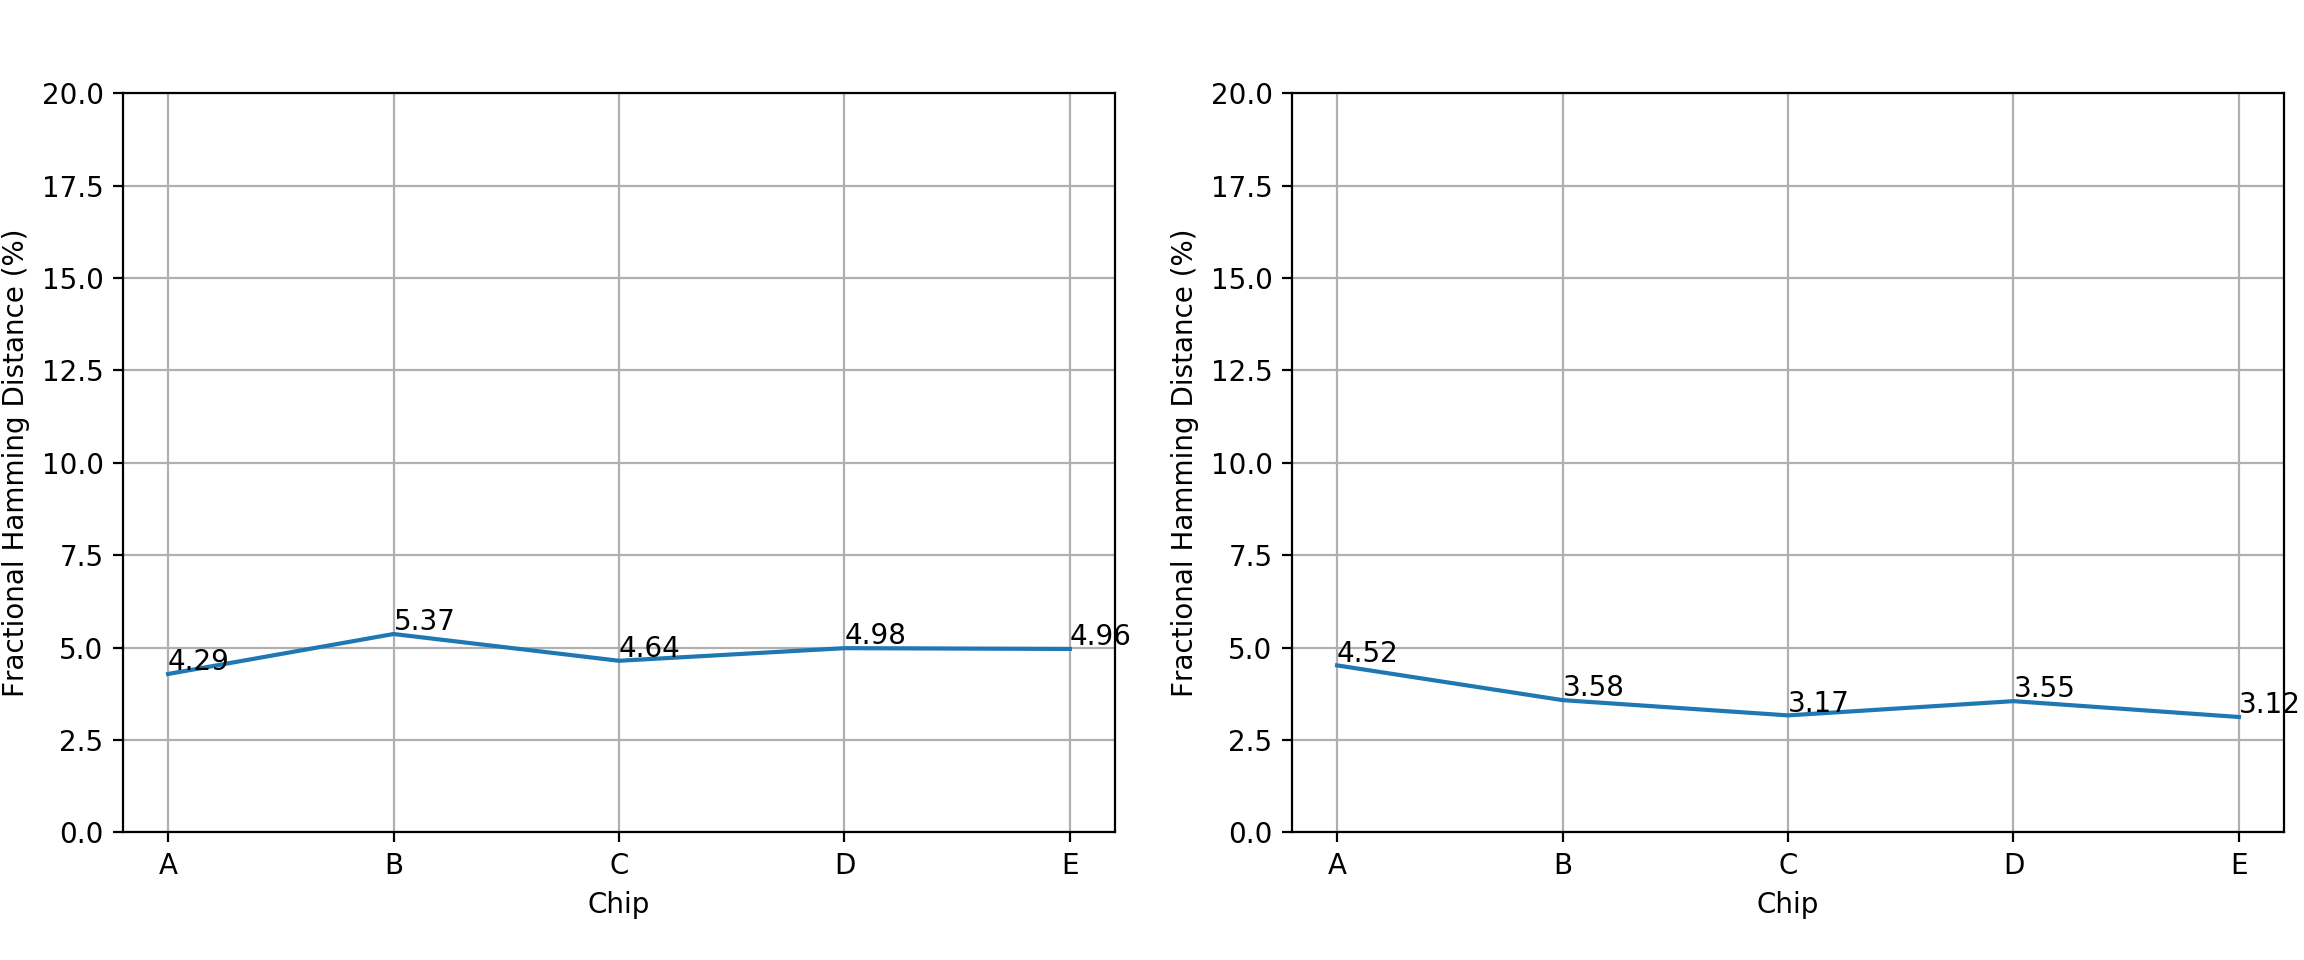
\includegraphics[width={\textwidth}]{images/cy62256nll_hd_intra}}
    \caption{HD\textsubscript{intra} of five SRAMs Cypress CY62256NLL. The left figure is the testing result of HD\textsubscript{intra} with constant voltage, the right one is tested based on the voltage variation.}
    \label{fig:cy62256nll_hd_intra}
\end{figure}

The results shown above indicate that SRAM Cypress CY62256NLL is a qualified candidate for SRAM PUF. A well distributed 0's and 1's inside SRAM memory, voltage variation has little effect on HD\textsubscript{intra} and HD\textsubscript{inter}, and no overlap between HD\textsubscript{intra} and HD\textsubscript{inter} lead us to continue using this SRAM on further experiments.

\section{Testing on Bit Selection Algorithms}

In this section, the test on stable bits produced by two algorithms, neighbor stability and data remanence analysis, is shown. The test was done on a single chip of each SRAM type.
% , one 23L1024 and one CY62256NLL.
The explanation of both algorithms can be found on section \ref{lbl:bit-selection}.

\subsection{Neighbour Stability Analysis}
To use this algorithm, first, data of SRAM bits value from various condition (voltages and time difference between data retrieval attempts) need to gathered. Afterwards, the bits which remained stable on all data retrieved are located. Then, the rank of remained stable bits are calculated. Last, n bits with highest rank can be used according to the necessity. The higher the rank, the more stable that bit should be.

\subsubsection{Microchip 23LC1024}
As input for the algorithm, there are 500 data of SRAM bits value used for this chip. The voltage variation is randomized between 2.5V - 5.0V. The time difference between data retrieval attempts is ranging from 5 seconds until 1 hour.
SRAM Microchip 23LC1024 itself has capacity 1048576 bits. After doing the calculation from those five hundred data, there are 413374 remaining stable bits. From those remaining stable bits, the rank of each bit is calculated. The frequency of bits rank is shown in Figure \ref{fig:23lc1024_score_rank_bits}. As shown in this figure, the total bits with rank more than 5 is insignificant, only showing 493 bits. Bits with rank more or equal to six is merged into a single bar because the frequency among those rank is usually only a single digit.

\begin{figure}[tph!]
    \centerline{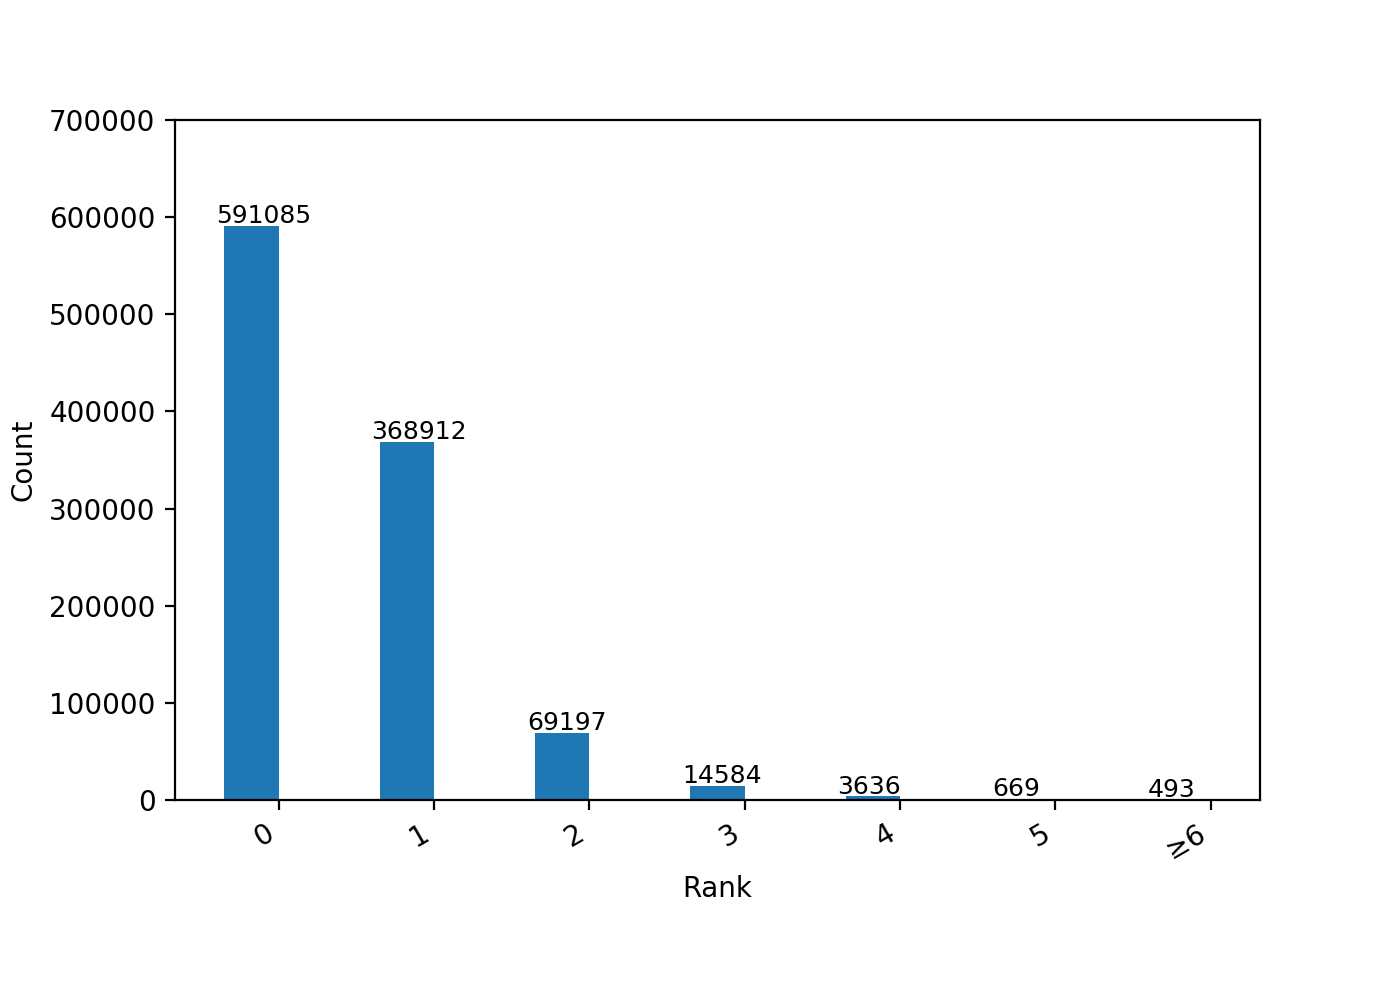
\includegraphics[width={0.9\textwidth}]{images/23lc1024_score_rank_bits}}
    \caption{Remaining stable bits count according to their rank in SRAM Microchip 23LC1024.}
    \label{fig:23lc1024_score_rank_bits}
\end{figure}

\subsubsection{Cypress CY62256NLL}
Similar like with SRAM Microchip 23LC1024, there are 500 memory values retrieved in SRAM Cypress CY62256NLL.
Cypress CY62256NLL is able to store 262144 bits in its memory. The remained stable bits after 500 data retrieval are 102708 bits (39,18\%).
The result of the calculation is shown on Figure \ref{fig:cy62256nll_score_rank_bits}. Compared to Microchip 23LC1024, this SRAM shows more promising result since there are many bits with ranks more than seven. Even to get two thousand bits, the lowest rank that can be included is twelve.

\begin{figure}[tph!]
    \centerline{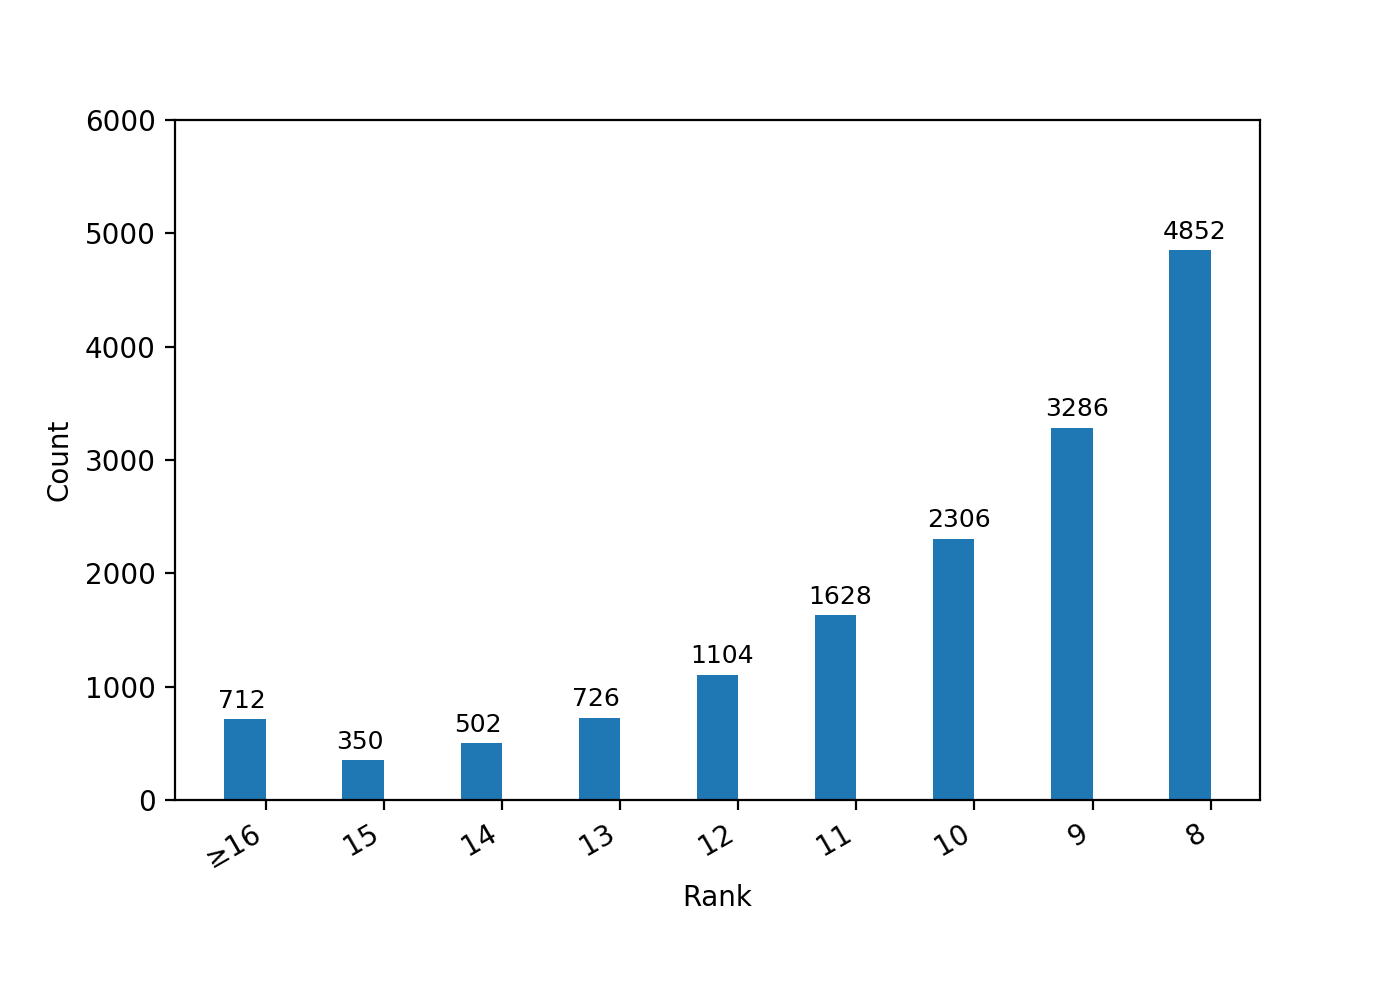
\includegraphics[width={0.9\textwidth}]{images/cy62256nll_score_rank_bits}}
    \caption{Remaining stable bits count according to their rank in SRAM Cypress CY62256NLL. There are 246678 bits with rank less or equal to seven.}
    \label{fig:cy62256nll_score_rank_bits}
\end{figure}

% \pagebreak
\subsection{Data Remanence Approach}

The result of data remanence analysis on both SRAMs is shown below.

\subsubsection{Microchip 23LC1024}

On SRAM Microchip 23LC1024, the data remanence analysis is done on time variance between 0-1.0 second. The result can be seen on Figure \ref{fig:23lc1024-remanence0}. In this figure, it is shown that
SRAM Microchip 23LC1024 will reach the uninitialized point if it is temporarily turn off for 0.7 seconds.

\begin{figure}[tph!]
    \centerline{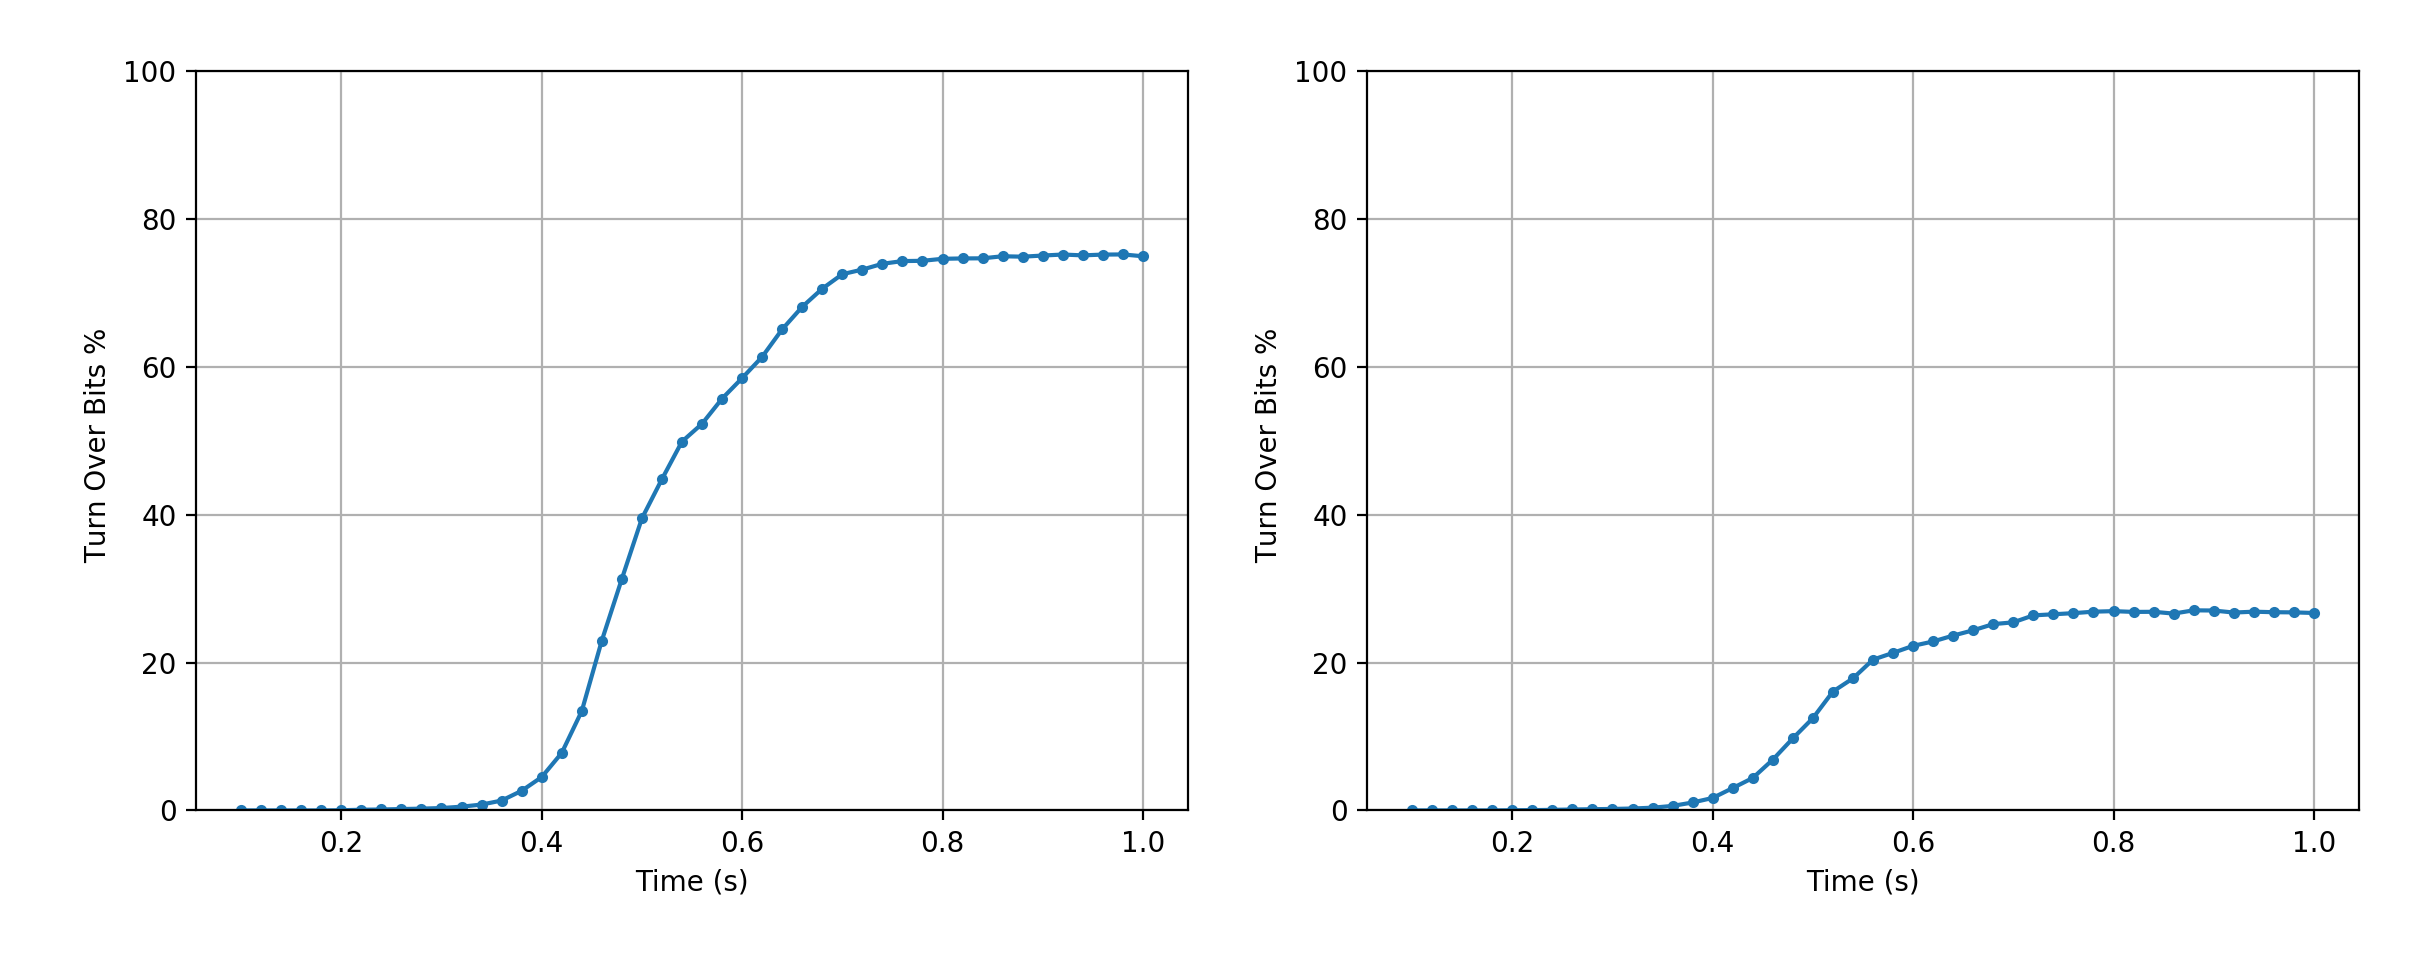
\includegraphics[width={\textwidth}]{images/remanence_23lc1024}}
    \caption{Measured SRAM Microchip 23LC1024 data remanence for data 0 (left) and data 1 (right).
    % Remanence Graph of SRAM Microchip 23LC1024. Left is remanence 0 and right is remanence 1.
    SRAM Microchip 23LC1024 will reach the uninitialized point if it is temporarily shut down for 0.7 second.}
    \label{fig:23lc1024-remanence0}
\end{figure}



\subsubsection{Cypress CY62256NLL}

On SRAM Cypress CY62256NLL, the data remanence analysis is done on time variance between 0-10 seconds. The result can be seen on Figure \ref{fig:23lc1024-remanence0}. In this figure, it is shown that
SRAM Cypress CY62256NLL will reach the uninitialized point if it is temporarily shut down for 5.0 second.

\begin{figure}[tph!]
    \centerline{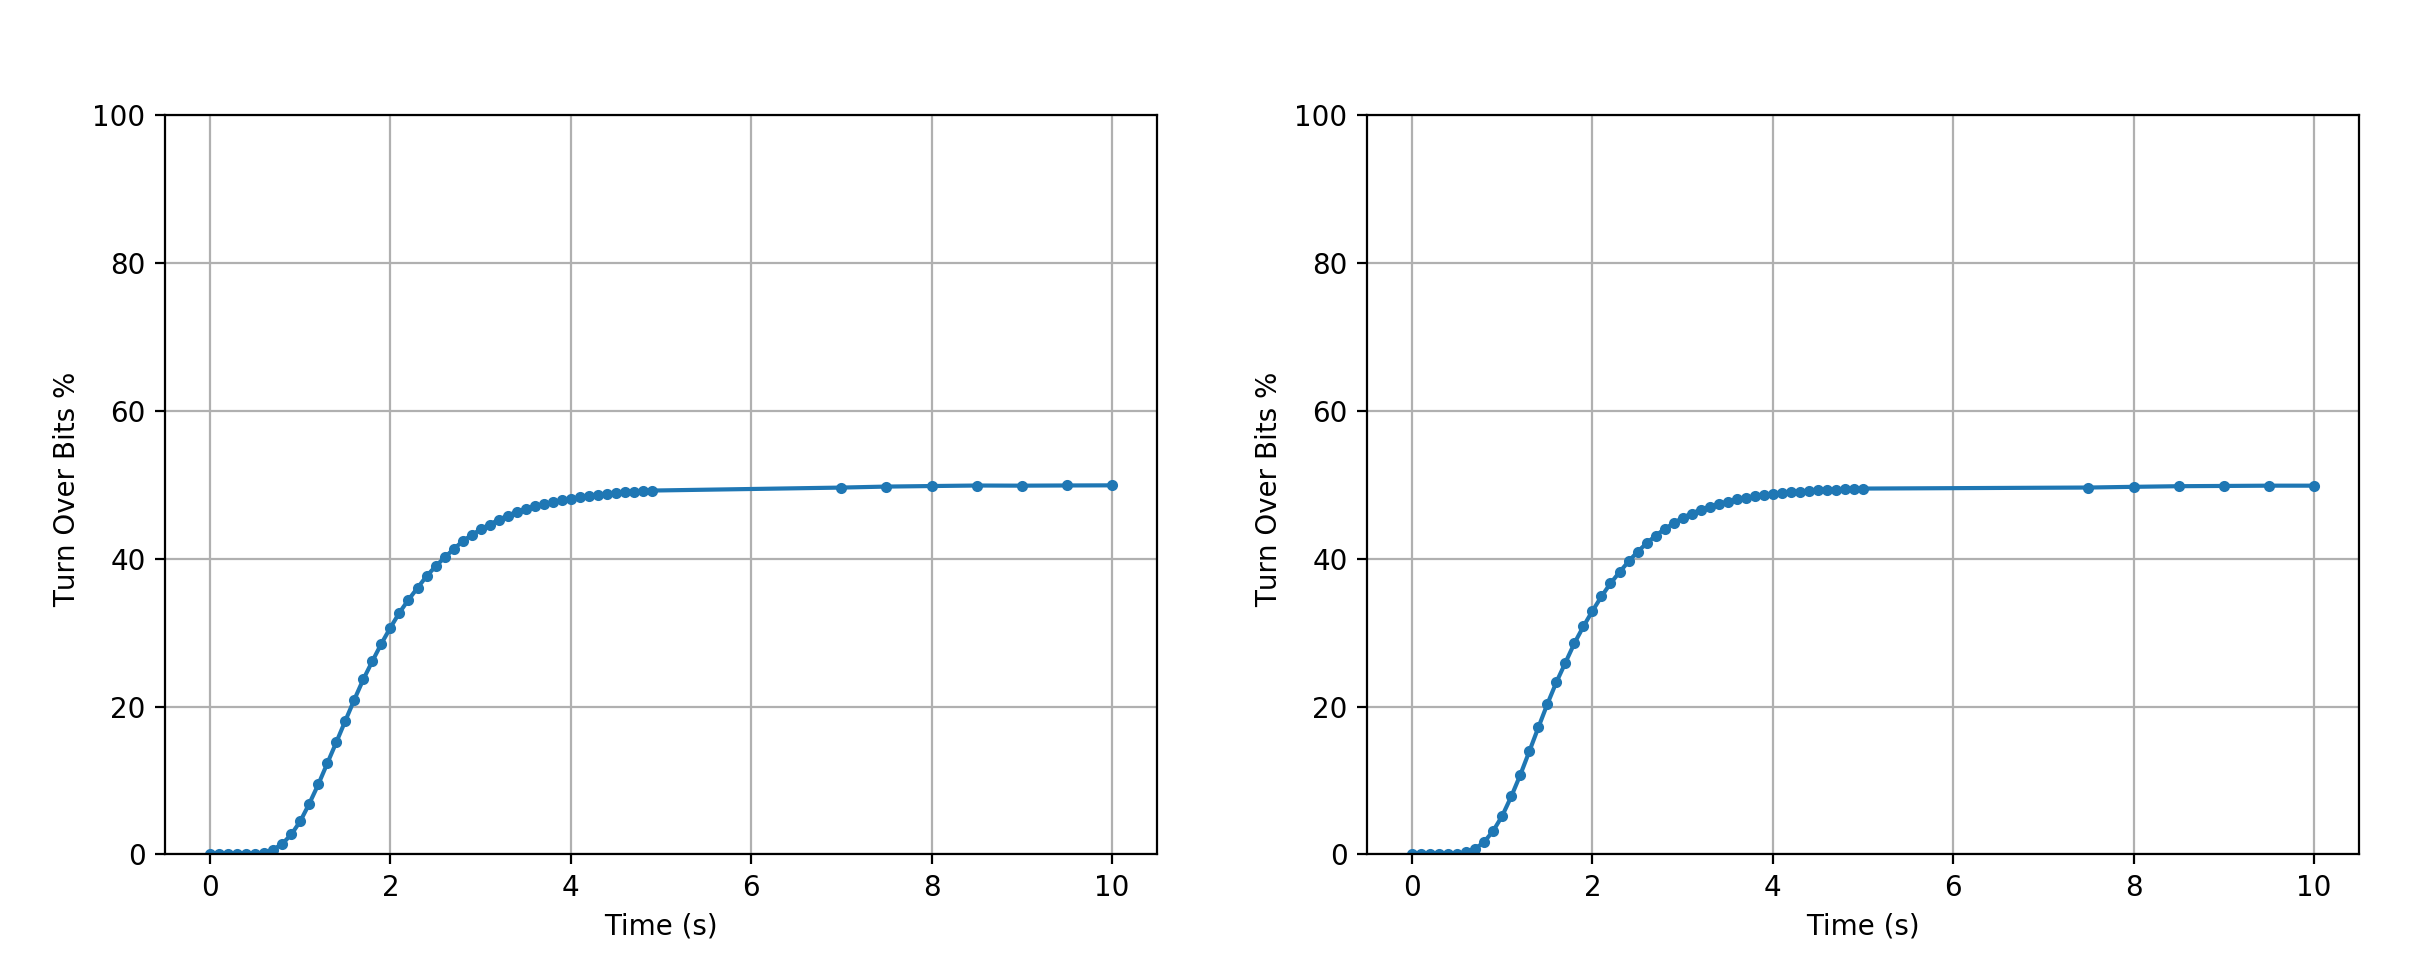
\includegraphics[width={\textwidth}]{images/remanence_cy62256nll}}
    \caption{Measured SRAM Cypress CY62256NLL data remanence for data 0 (left) and data 1 (right).
    % Remanence Graph of CY62256NLL. Left is remanence 0 and right is remanence 1.
    SRAM Cypress CY62256NLL will reach the uninitialized point if it is temporarily shut down for 5.0 second.}
    \label{fig:CY62256NLL-remanence0}
\end{figure}


\subsection{Stability Test on Stable Bits}\label{ch:hd_intra_stable}
In this section, test results on the effect of time interval and voltage on stable bits using both algorithms on each SRAM are shown. The effect of aging and temperature is not tested due to a limitation on time and equipment. For the effect of time interval testing, the enrollment was done on 16 days with one day gap between enrollment. Voltage effect testing was done on voltage ranging from 4.5V-5V for SRAM Cypress CY62256NLL and 2.5V-5V for SRAM Microchip 23LC1024. The test is done on 4662 bits which is twice the length of the bits required to generate 256 bits key when using scheme shown in Figure \ref{fig:key-generation-scheme}. The result of time interval testing on SRAM Microchip 23LC1024 is shown on Figure \ref{fig:test_stable_23lc1024}, while Figure \ref{fig:test_stable_cy62256nll} displays the result for SRAM Cypress CY62256NLL.

\begin{figure}[tph!]
    \centerline{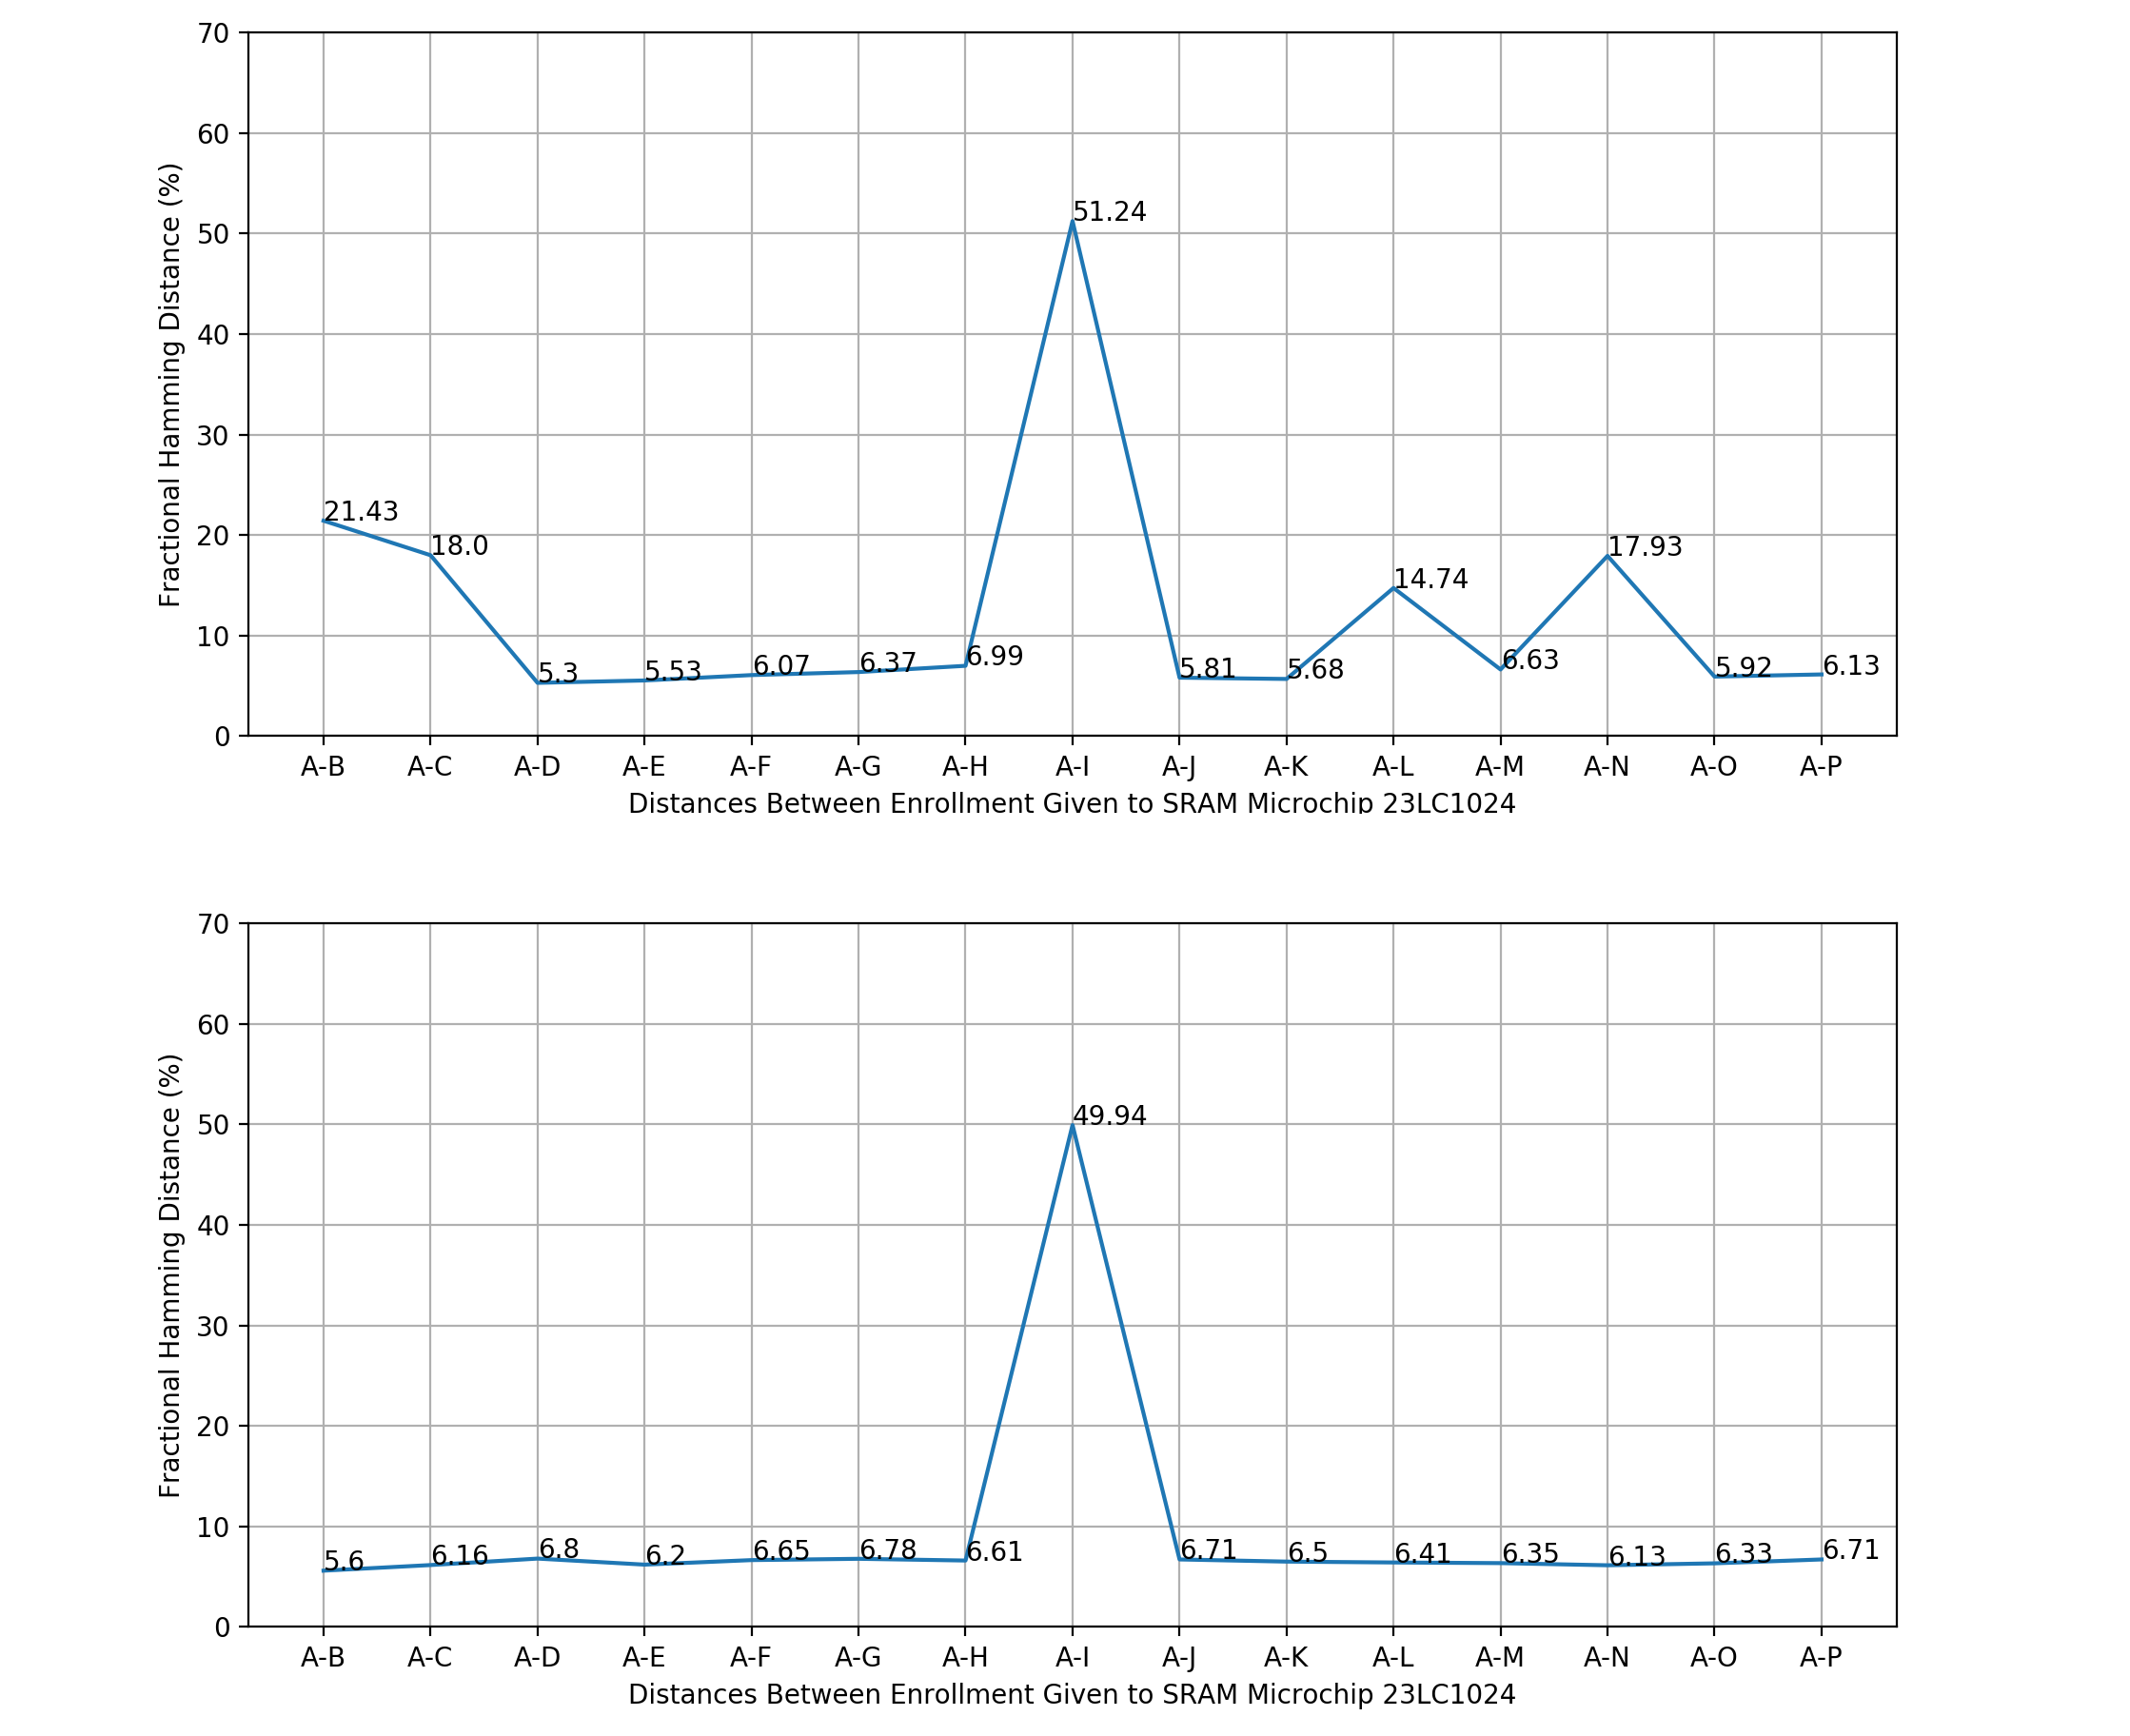
\includegraphics[width={1.1\textwidth}]{images/23lc1024_hd_intra_time_stable}}
    \caption{Time interval testing results on SRAM Microchip 23LC1024. Top figure is the testing result on stable bits generated using neighbor analysis, while the bottom one is tested on data remanence generated stable bits. Index A on x-axis refers to enrollment on day 1, B on day 2, etc. Index A-B refers to fractional hamming distance between enrollment on day 1 and day 2.}
    \label{fig:test_stable_23lc1024}
\end{figure}

\begin{figure}[tph!]
    \centerline{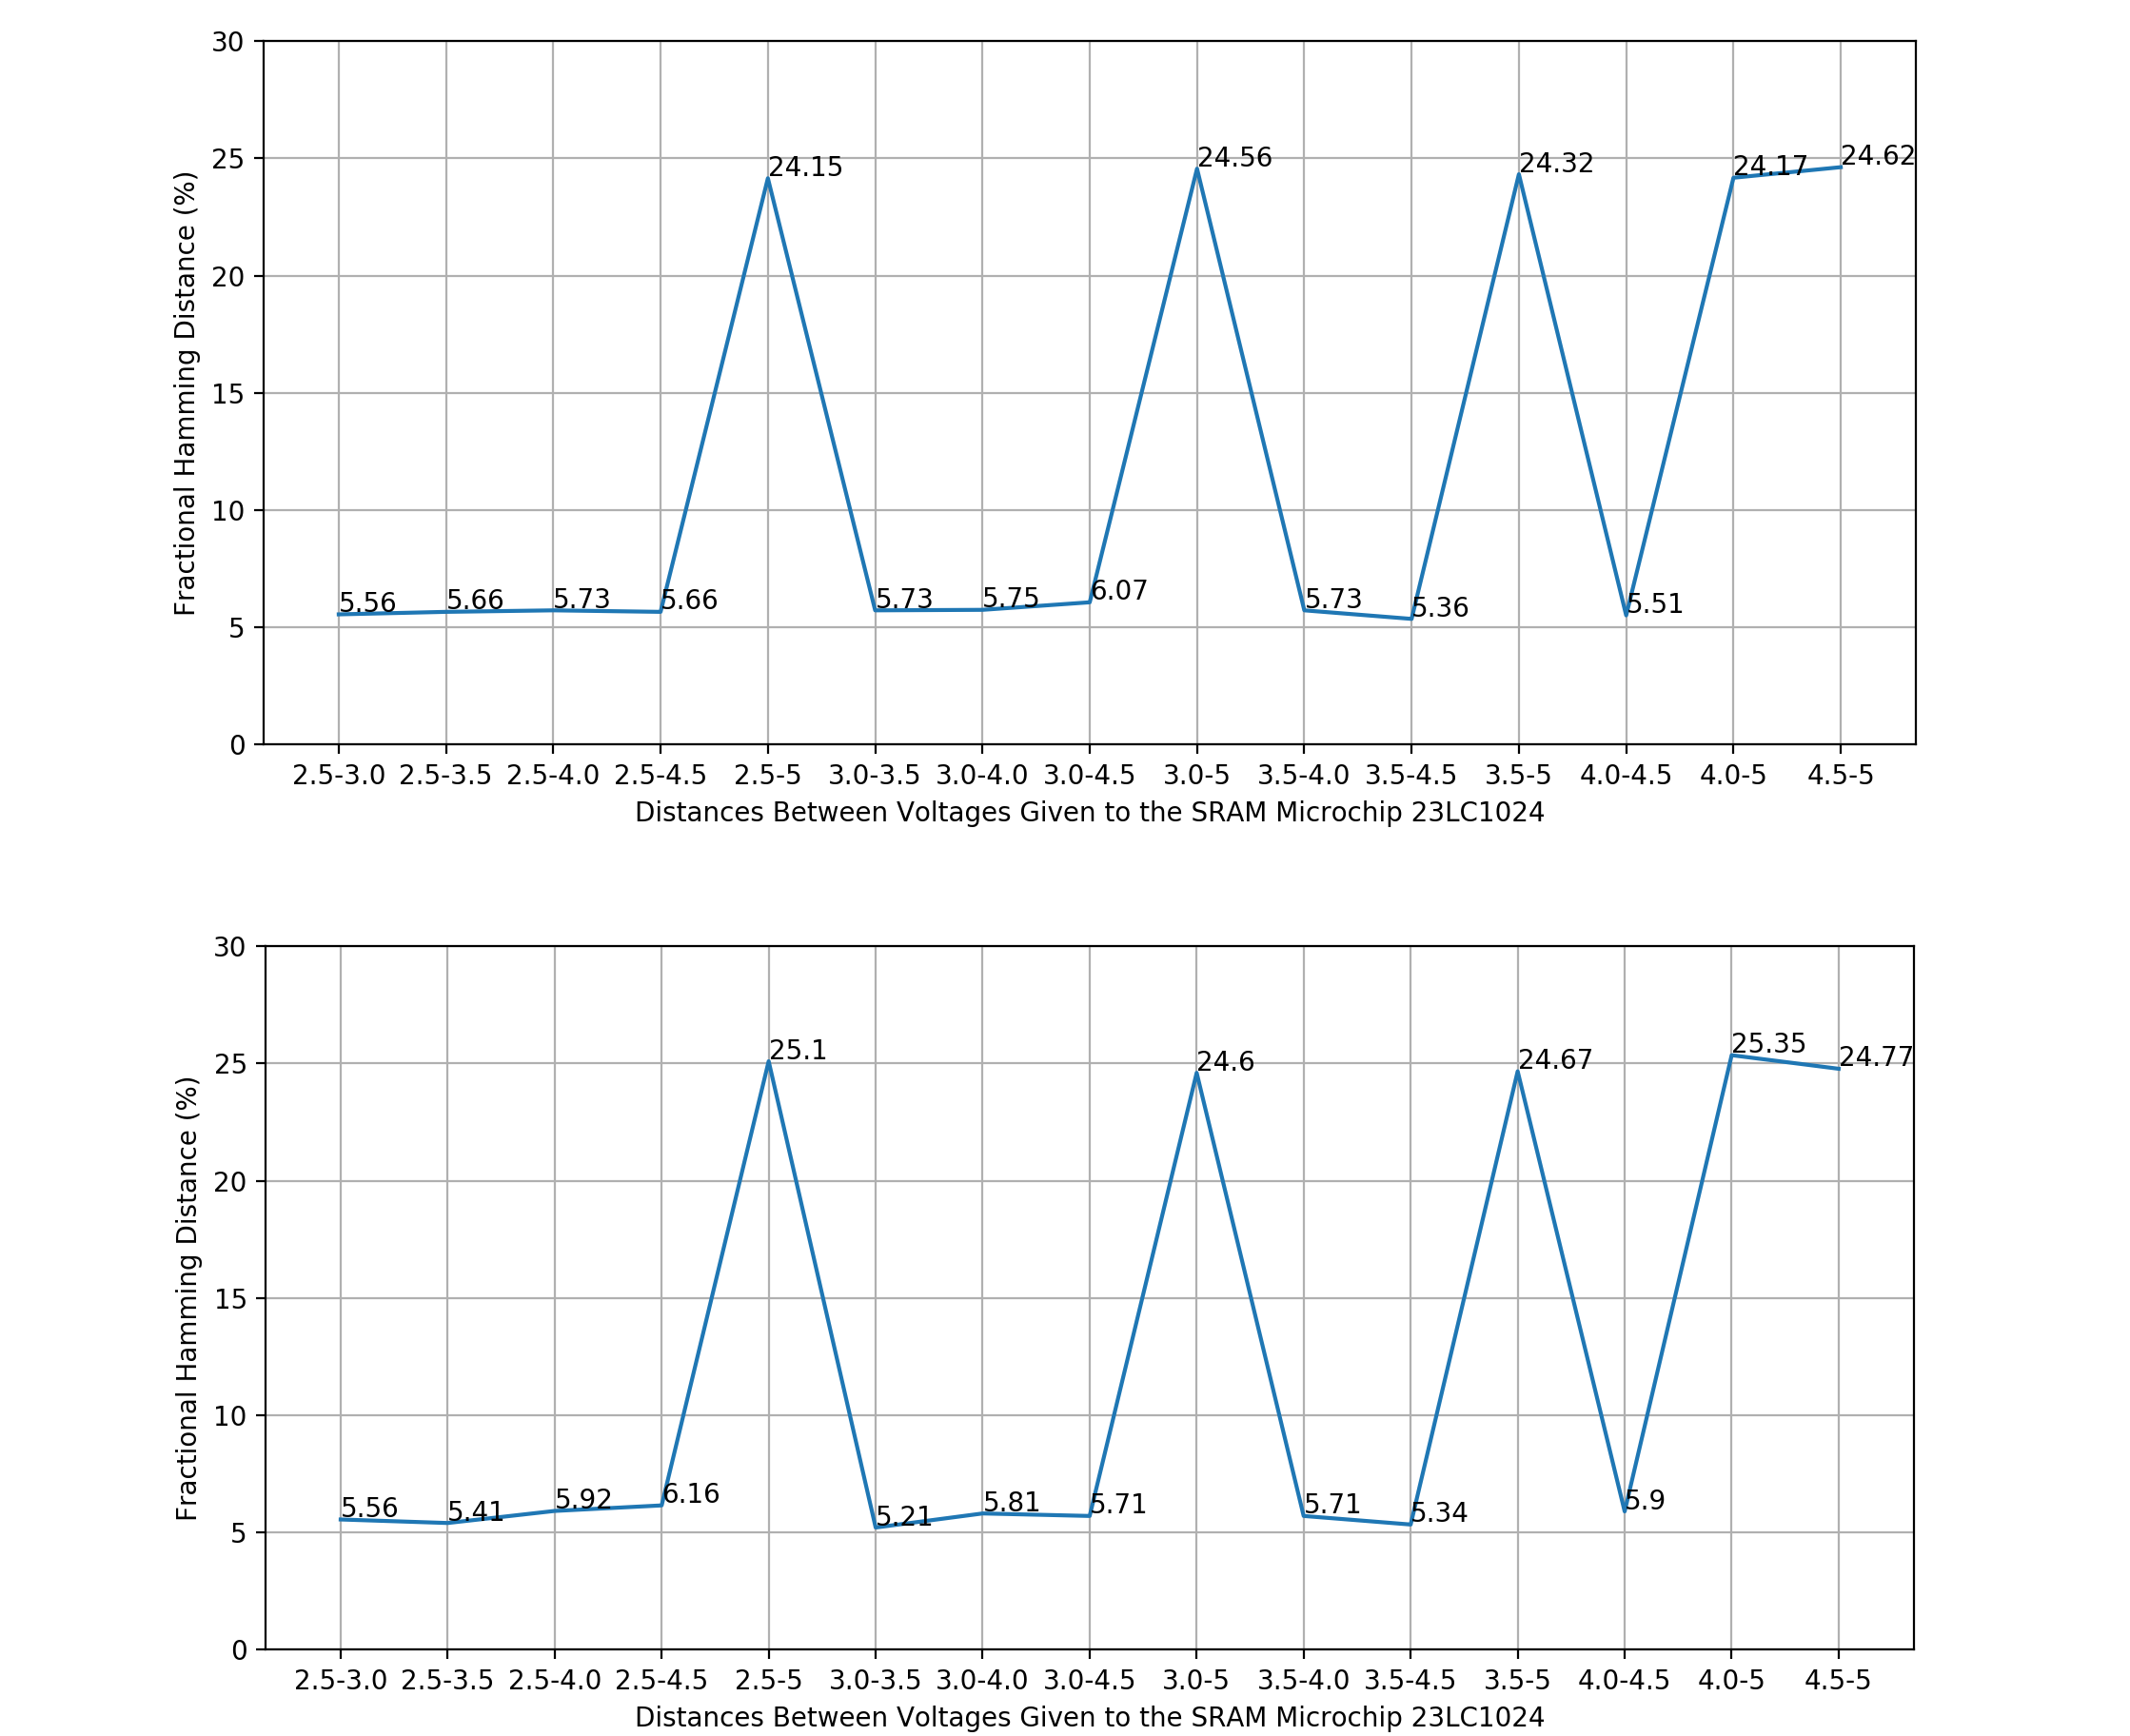
\includegraphics[width={1.1\textwidth}]{images/23lc1024_hd_intra_voltage_stable}}
    \caption{Voltage variation testing results on SRAM Microchip 23LC1024. Top figure is the testing result on stable bits generated using neighbor analysis, while the bottom one is tested on stable bits produced by data remanence analysis. Index on x-axis refers to two different voltages, e.g. 2.5-5.0 means the fractional hamming distance between enrollment on voltage 2.5V and voltage 5.0V.}
    \label{fig:test_stable_23lc1024_voltage}
\end{figure}

\begin{figure}[tph!]
    \centerline{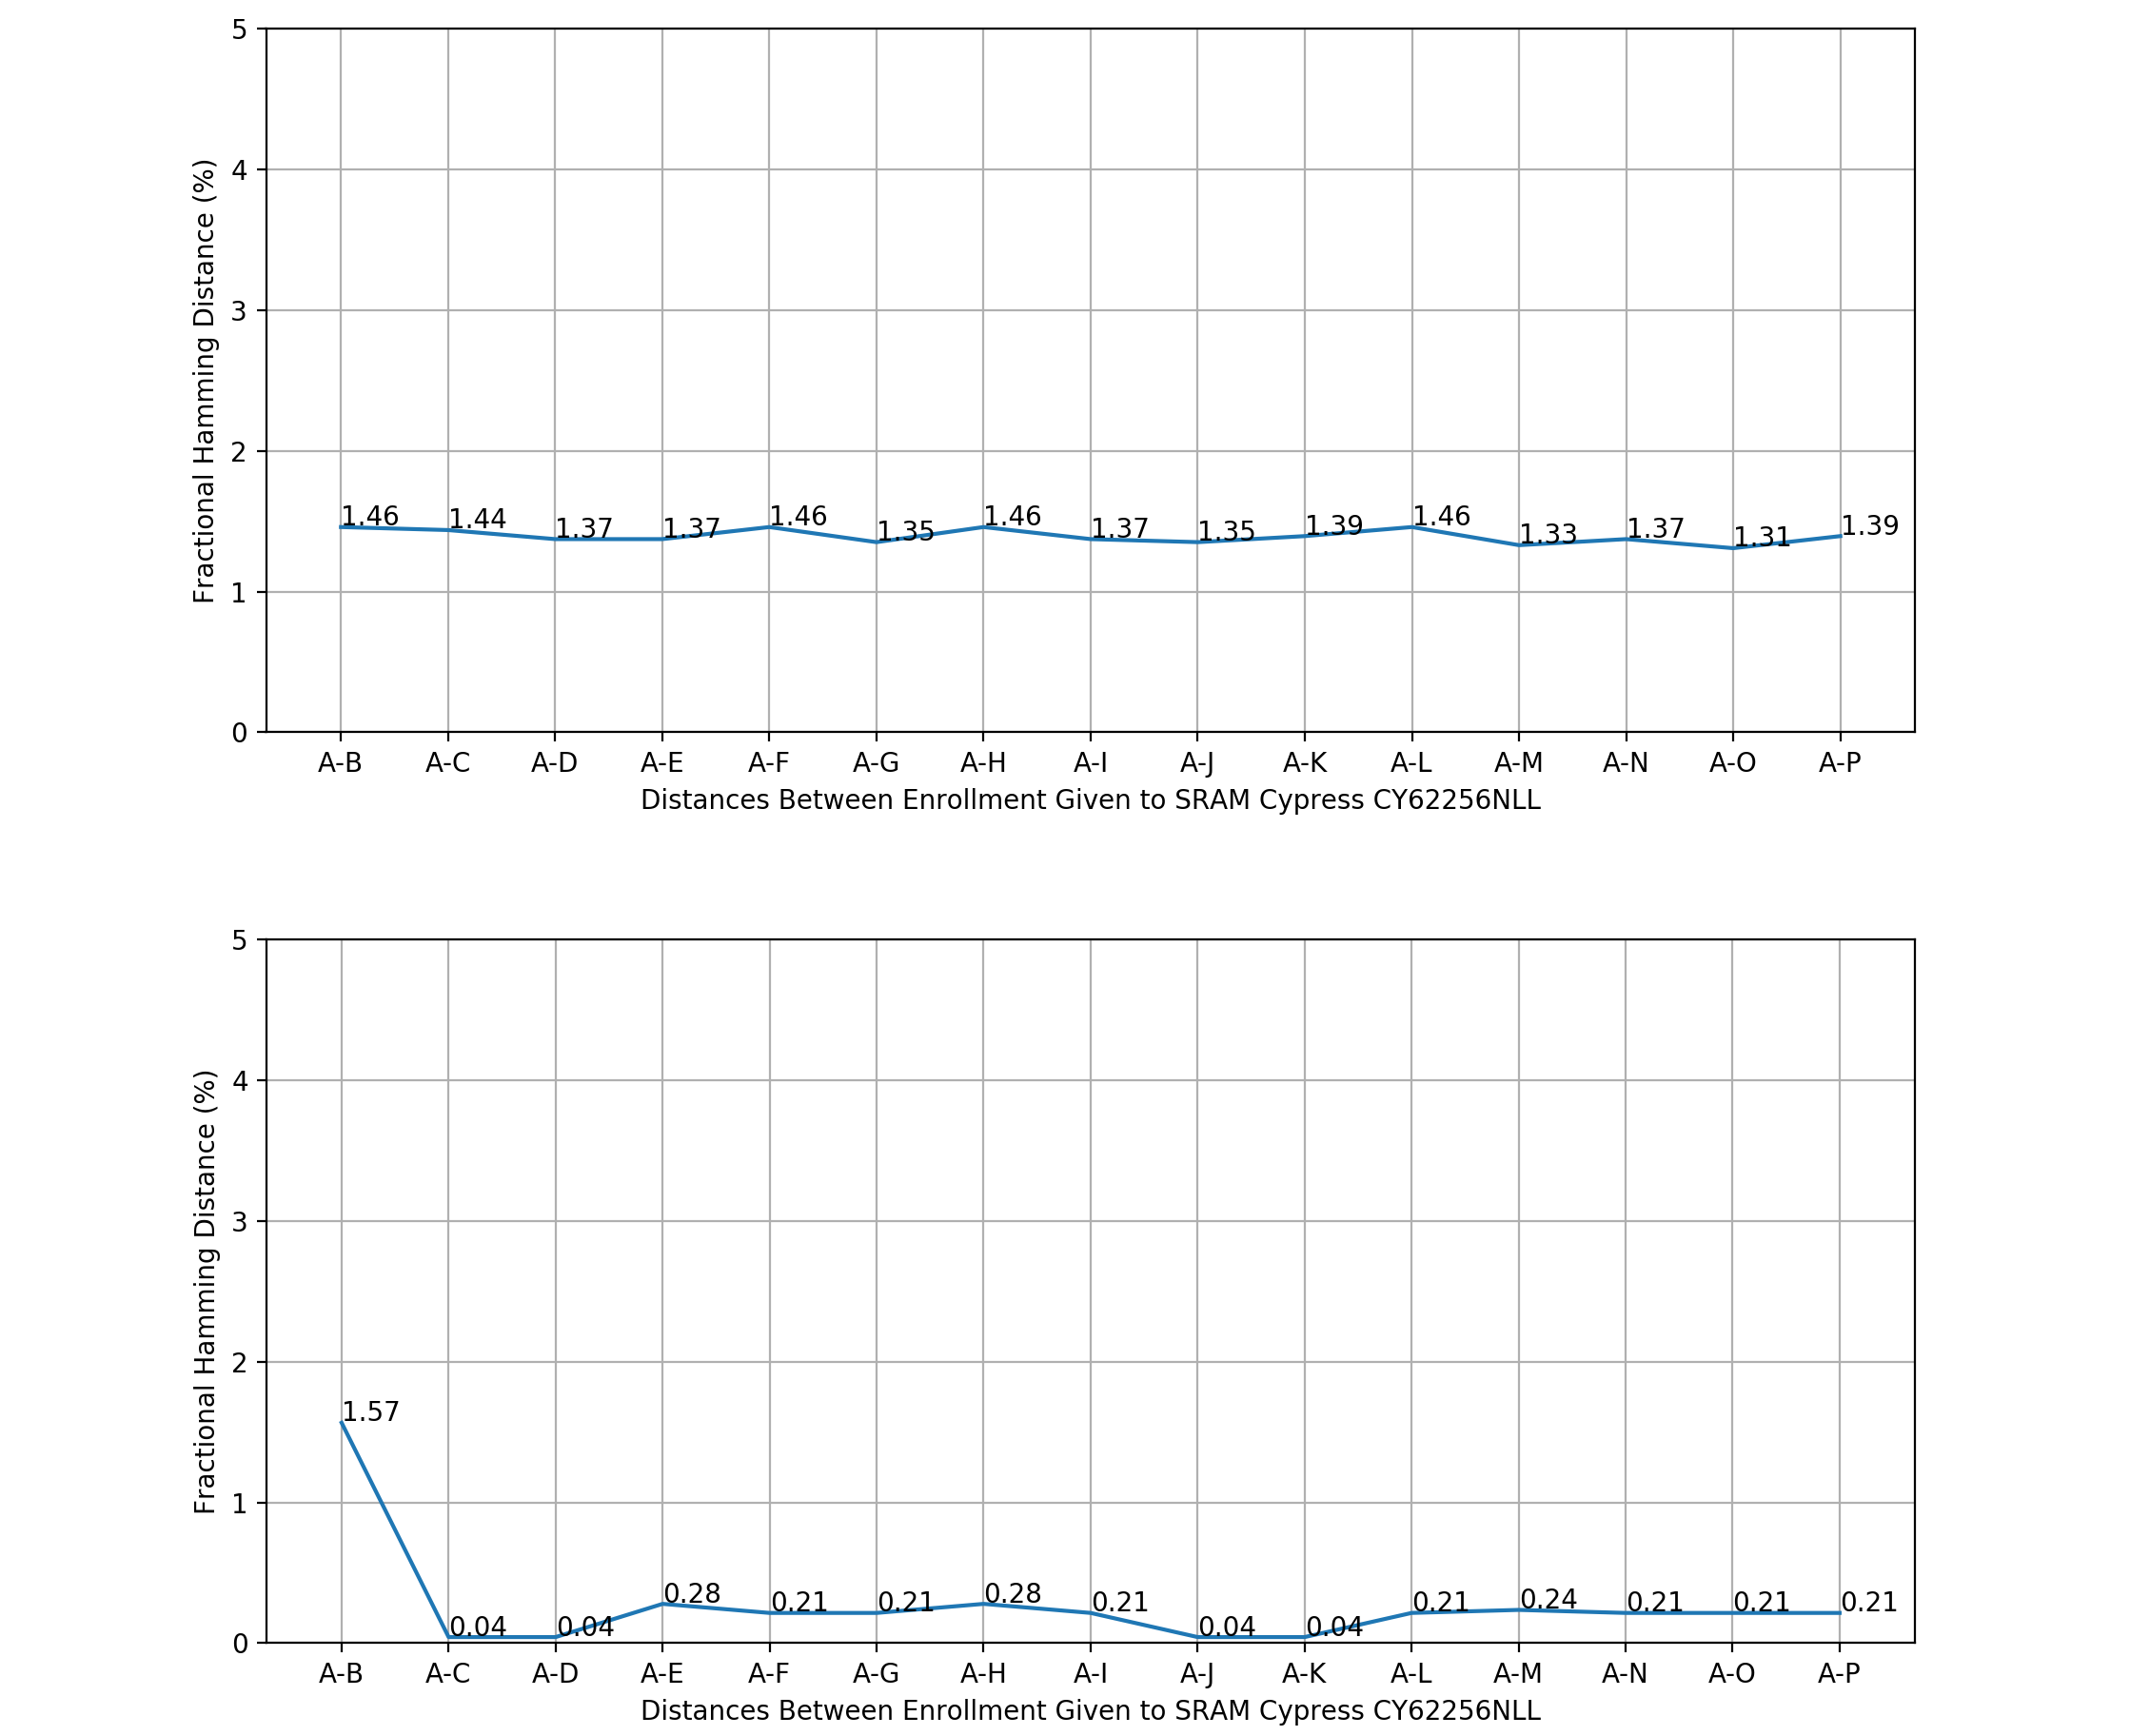
\includegraphics[width={1.1\textwidth}]{images/cy62256nll_hd_intra_time_stable}}
    \caption{Time interval testing results on SRAM Cypress CY62256NLL. Top figure is the testing result on stable bits generated using neighbor analysis, while the bottom one is tested on data remanence generated stable bits. Index A on x-axis refers to enrollment on day 1, B on day 2, etc. Index A-B refers to fractional hamming distance between enrollment on day 1 and day 2.}
    \label{fig:test_stable_cy62256nll}
\end{figure}

\begin{figure}[tph!]
    \centerline{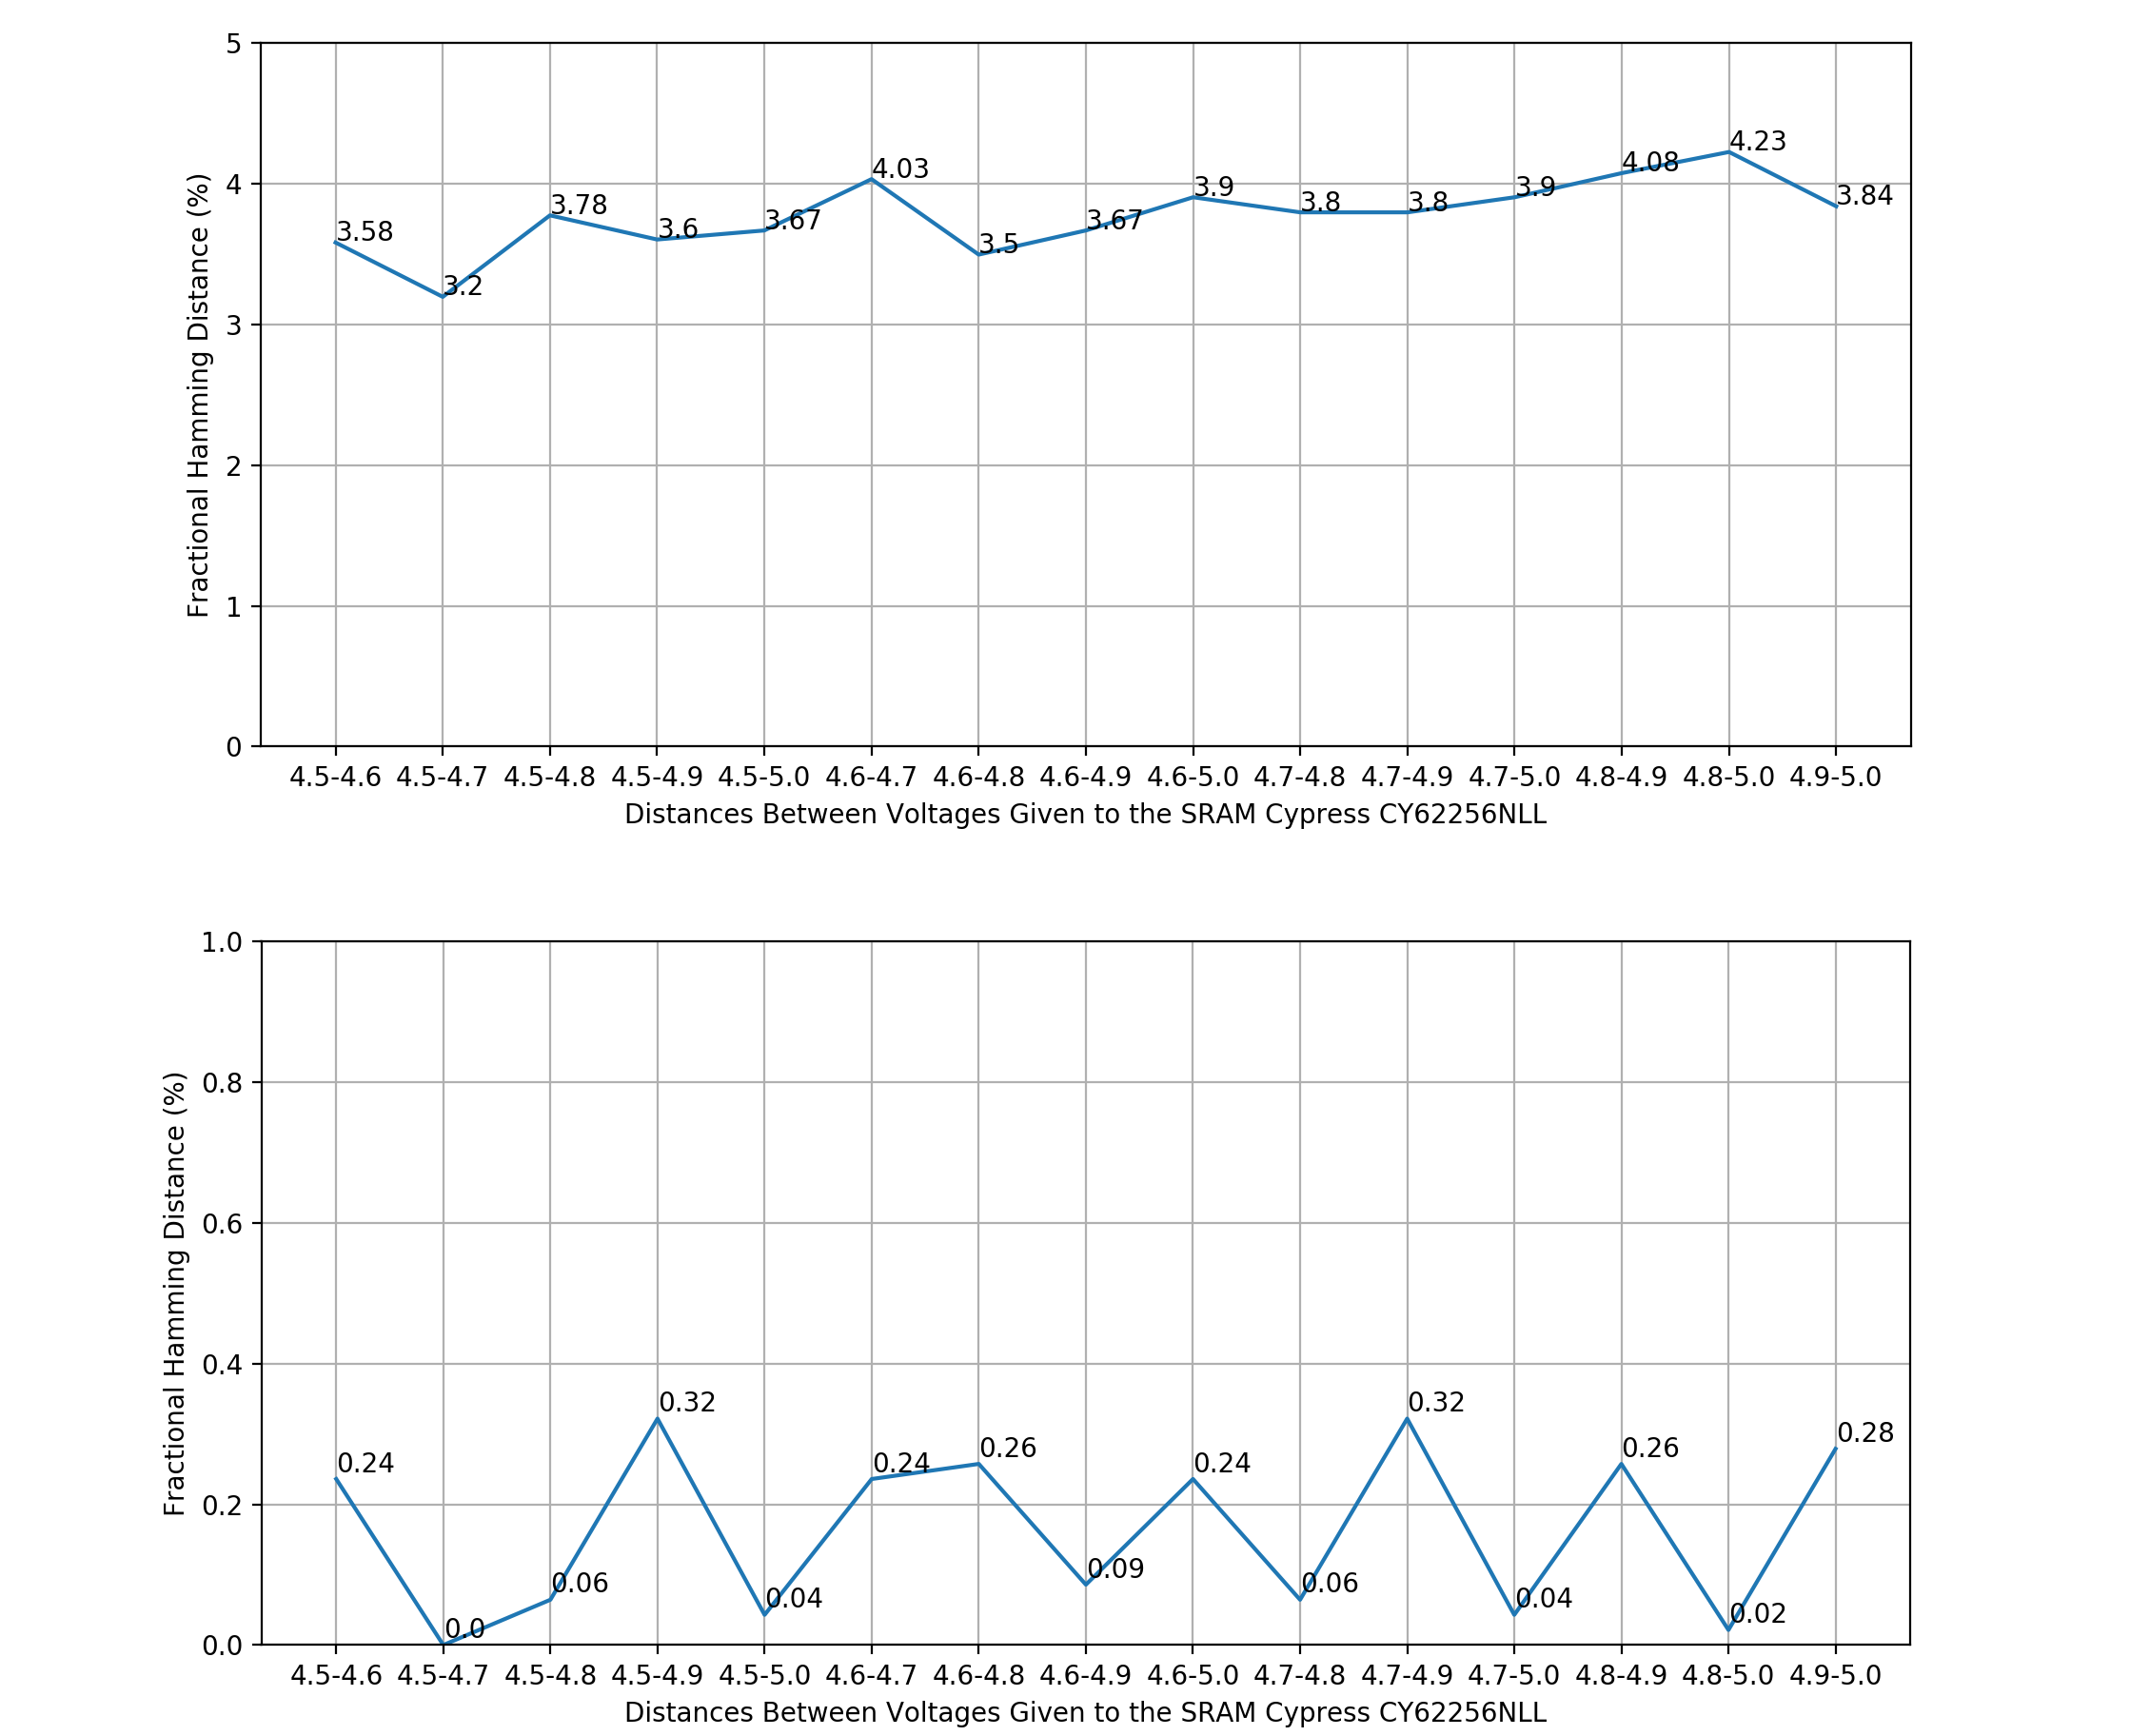
\includegraphics[width={1.1\textwidth}]{images/cy62256nll_hd_intra_voltage_stable}}
    \caption{Voltage variation testing results on SRAM Cypress CY62256NLL. Top figure is the testing result on stable bits generated using neighbor analysis, while the bottom one is tested on stable bits produced by data remanence analysis. Index on x-axis refers to two different voltages, e.g. 4.5-4.6 means the fractional hamming distance between enrollment on voltage 4.5V and voltage 4.6V.}
    \label{fig:test_stable_cy62256nll_voltage}
\end{figure}

\subsubsection{Microchip 23LC1024}
\begin{itemize}
  \item Neighbor Stability Analysis\newline
  To get 4662 bits, there are three categories included; rank similar or higher than 6 with 493 bits, rank 5 with 669 bits, and rank 4 with 3500 bits.
  During testing on variated voltage and time interval, the stable bits generated using neighbor stability analysis show a poor performance by having maximum 2389 bits changing  (HD\textsubscript{intra} 51.24\%) which also produces an overlap between HD\textsubscript{intra} and HD\textsubscript{inter}. The maximum difference is produced when the difference between enrollment is 8 days.

  \item Data Remanence Approach\newline
  To get 4662 bits, strong 1's are generated using power down period of 0.185 seconds, while strong 0's are calculated when 0.27 seconds are used as the power down period. The difference between power down period during generation of strong 1's and strong 0's is because the number of 1's that flipped fast are more compared to 0's. This is also related to the 0's and 1's distribution during normal initialization (0's count for 30\% and 1's filled 70\%).
  Similar to the previous algorithm, the stability of bits produced by using this algorithm is also not good. The worst change happens when 8 days is used as the time interval between testing, showing as many as 2328 bits (HD\textsubscript{intra} 49.93\%) and also introduce an overlap between HD\textsubscript{intra} and HD\textsubscript{inter}.
\end{itemize}

\subsubsection{Cypress CY62256NLL}
\begin{itemize}
  \item Neighbor Stability Analysis\newline
  To get 4662 bits, there are six categories included; rank similar or higher than 16 with 712 bits, rank 15 with 350 bits, rank 14 with 502 bits, 726 bits of rank 13, 1104 bits of rank 12, and 1268 bits of rank 11.
  Under the voltage and time interval variation, the stable bits generated using neighbor stability analysis show decent reliability by having maximum 197 changing bits (HD\textsubscript{intra} 4.23\%) when the data is gathered on voltage 4.8V and 5V.

  \item Data Remanence Approach\newline
  Unlike SRAM 23LC1024, power down period when enrolling strong 1's and 0's on CY62256NLL is not different. To get 4662 stable bits, both are enrolled using power down period 0.34 seconds.
  During the voltage and time interval variation, the stable bits produced by using algorithm also shows a promising result. It only accounts for maximum 73 bits difference (HD\textsubscript{intra} 1.56\%).
\end{itemize}


\subsubsection{Stability Test Conclusion}

Based on these results, SRAM Cypress CY62256NLL is shown to be a reliable SRAM candidate for PUF due to its well distribution of 1's 0's inside its memory and small variance when tested on various voltage and time interval between enrollment, especially the stable bits produced by data remanence analysis which has HD\textsubscript{intra} less than 2\% on any testing. If Cypress CY62256NLL is used as the root-of-trust to produce PUF-generated key, the key is ensured to always have the same value since the key generation scheme can tolerate up to 12.7\% while the error rate of stable bits of Cypress CY62256NLL produced by data remanence algorithm is always less than 2\%.
Sadly, the other SRAM, SRAM Microchip 23LC1024, has displayed a poor performance to be eligible as a PUF candidate. Unbalanced 1's and 0's distribution and large HD\textsubscript{intra} when the stable bits are tested (larger than the maximum error capability of the key generation scheme, and even introduces an overlap between HD\textsubscript{intra} and HD\textsubscript{inter}) are two main reasons why this SRAM is not recommended to use as a PUF candidate.

These different results between two types of SRAMs lead us to a thinking that the SRAM size and the technology used in SRAM manufacturing affects a lot of SRAM quality as a PUF candidate. For example, Cypress CY62256NLL has significantly larger size than Microchip 23LC1024 (a rough approximation results in 13.38 times larger). Cypress CY62256NLL also has a smaller capacity (256k) than Microchip 23LC1024 (1024k). In addition, Cypress CY62256NLL is produced using an older technology (90nm) compared to Microchip 23LC1024 which has a higher chance to be produced using a newer technology since it has a much smaller size but larger memory size than Cypress CY62256NLL (there is no information on manufacturing technology used in the production on their websites and the Microchip 23LC1024 manual descriptions). From these explanations, we can conclude that Cypress CY62256NLL has less density than Microchip 23LC1024. These reasons lead us to a confirmation of density effects  explained in Section \ref{ch:sram_noise} which says the more dense an SRAM, the more environments affect the performance of the SRAM. But does it mean that SRAM PUF cannot be produced using an SRAM with a high density? This seems untrue due to some SRAM PUF references mentioned a newer technology in their PUF constructions, e.g. Cortez et. al. in \cite{7102498} use SRAMs which produced using 32nm and 45nm (sadly, there is no information on the type and manufacturer of their tested SRAMs). Moreover, as mentioned in Section \ref{ch:prev_experiments}, the experiments done in \cite{Schrijen:2012:CAS:2492708.2493033} shown that an older manufacturing technology doesn't always produced a more stable SRAM (Cypress CY7C15632KV18 (65nm) is more stable than Virage HP ASAP SP ULP 32-bit (90nm), even though the most stable is IDT 71V416S15PHI which produced using 180nm technology).
Furthermore, since every company always has their own way of dealing with noises introduced by high density level, we cannot conclude that high density level always lead to low quality of an SRAM as a PUF candidate. Now, this lead to another questions, what is the main criteria if an off-the-shelf SRAM is going to be used a PUF candidate? Should we trust specific company such as Cypress and mistrust another company like Microchip? Or do we need to look into specific product to determine whether an SRAM is suitable for a PUF component? Should we always prefer SRAMs with less density?
% Now, this also brings to other questions, what is the optimum density for an off-the-shelf SRAM to be valid as a PUF candidate?
We suggest the communities and the academics to study this thing further.

Another conclusion that can be retrieved is that data remanence analysis is also proven to be a better bit selection algorithm than neighbor analysis which also confirms similar claim by Muqing et. al. \cite{liu_zhou_tang_parhi_kim_2017}. Futhermore, based on this outcome, further testing shown below are only done on SRAM Cypress CY62256NLL and the stable bits used are generated using the data remanence algorithm.

\section{Testing on Bits Locations as A Challenge}
In this section, the testing results on our proposed PUF challenge is presented. As mentioned in the previous chapter, bits locations is selected as the PUF challenge in our application. The test was done on SRAM Cypress CY62256NLL. Cypress CY62256NLL itself has a capacity to store 262144 bits. The number of bits required in a challenge is 2331 bits (the length of the bits required to generate 256 bits key when using scheme shown in Figure \ref{fig:key-generation-scheme}). Using Equation \ref{bits} explained in previous chapter, there are $P(262144, 2331)=\frac{262144!}{\left( 262144-2331 \right) !}\approx 10^{12626}$ possible combinations.

The selected test to test this challenge is by calculating the HD\textsubscript{inter} among five SRAMs. Figure \ref{fig:cy62256cy62256nll_hd_inter_stable_remanences} shows the result of this experiment. As shown in that figure, the HD\textsubscript{inter} is ranging between 35.26\% until 46.93\%, with average 42.08\%. Since there is no overlap between HD\textsubscript{intra} (shown on Section \ref{ch:hd_intra_stable}) and HD\textsubscript{inter}, this result shows that using bits locations as a challenge is sufficient to distinguish an SRAM from another.

\begin{figure}[tph!]
    \centerline{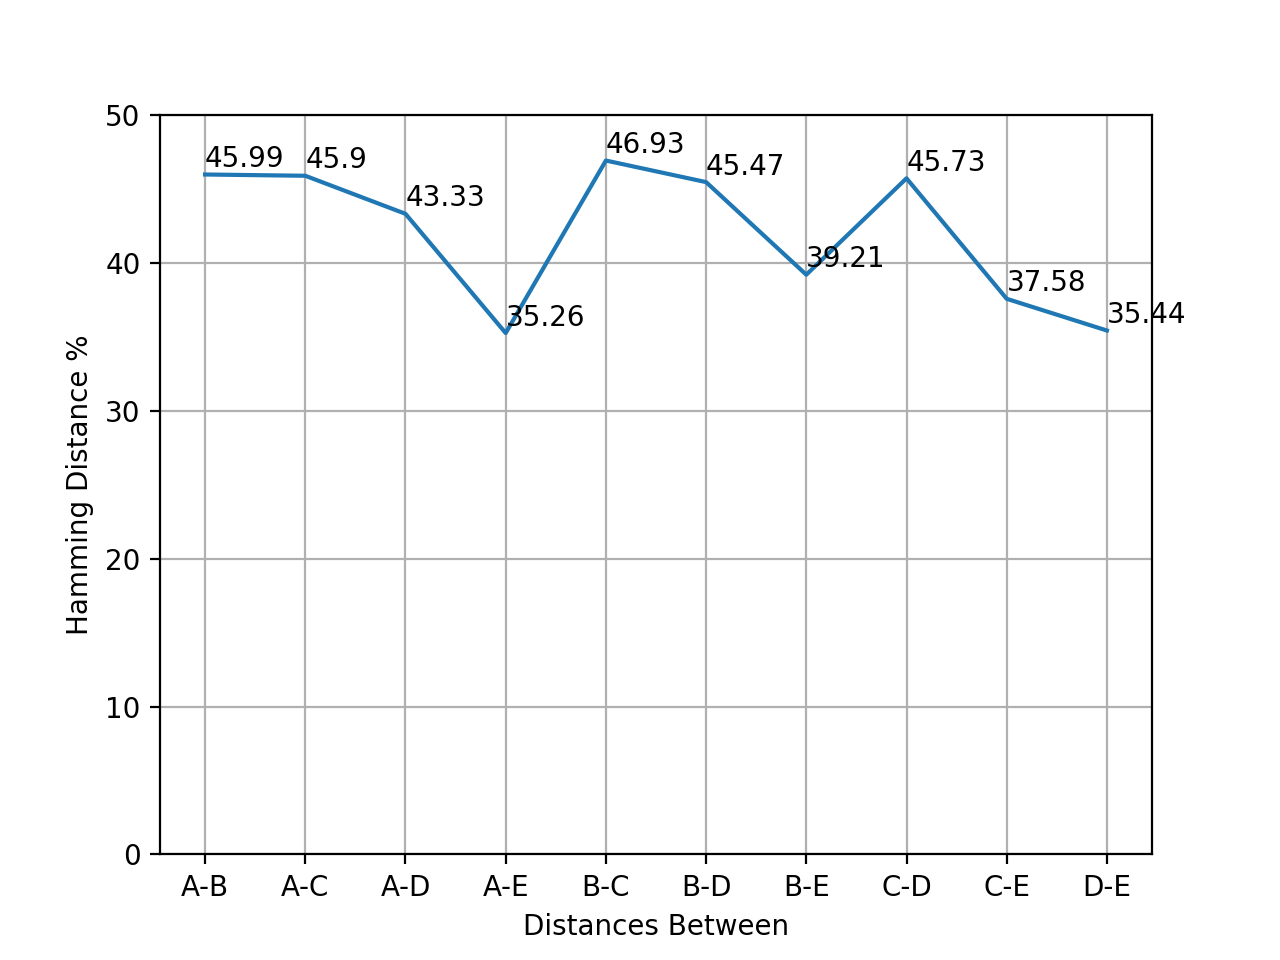
\includegraphics[width={0.9\textwidth}]{images/cy62256nll_hd_inter_stable_remanences}}
    \caption{HD\textsubscript{inter} among five SRAMs Cypress CY62256NLL. }
    \label{fig:cy62256cy62256nll_hd_inter_stable_remanences}
\end{figure}

\section{Complete Enrollment Scheme}\label{ch:complete_enrollment_scheme}
Based on the experiment results shown before, we construct a complete enrollment scheme. The enrollment scheme has a goal to create challenge and helper data which will be used in our proposed secure data protection and key storage scheme (further explanation is available on Section \ref{chp:data_protection_scheme}).
Similar to the automatic profiling system, the enrollment scheme also consists of a PC, act as a master, and an Arduino connected to an external SRAM component which acts as a slave. The PC side will run Python code while Arduino side requires Arduino code.
Our complete enrollment scheme is shown in Figure \ref{fig:enrollment}. We also present Figure \ref{fig:cy62256nll_scheme_sd} to show how to connect an Arduino Mega 2560, an SRAM Cypress CY62256NLL and a microSD.

The enrollment scheme starts by locating stable bits using bit selection algorithm. The chosen bit selection algorithm is data remanence analysis due to its better result and shorter time needed compared to neighbor analysis. Using this algorithm, we detect the position of 4662 stable bits. Afterwards, these stable bits are shuffled to form a set of 2331 bits locations which will be used as the PUF challenge. The process continues with creating the helper data based on the PUF challenge. The enrollment scheme ends with storing the helper data and the PUF challenge to a microSD. Later, if one wants to reconstruct the PUF-generated key from the helper data and the challenge, he only requires an Arduino, no PC is needed (the Arduino code used for reconstructing the PUF-generated key is different from the Arduino code when it act as a slave).

\begin{figure}[tph!]
    \centerline{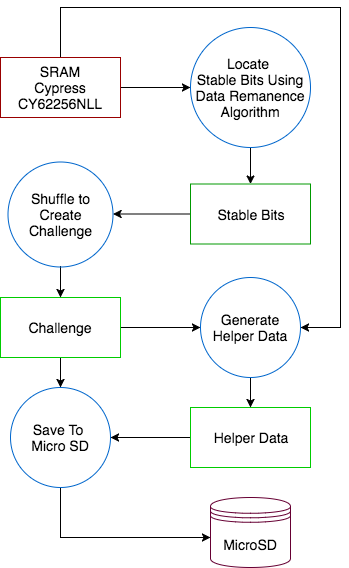
\includegraphics[width={0.5\textwidth}]{images/enrollment}}
    \caption{Complete enrollment setup.}
    \label{fig:enrollment}
\end{figure}

\begin{figure}[tph!]
    \centerline{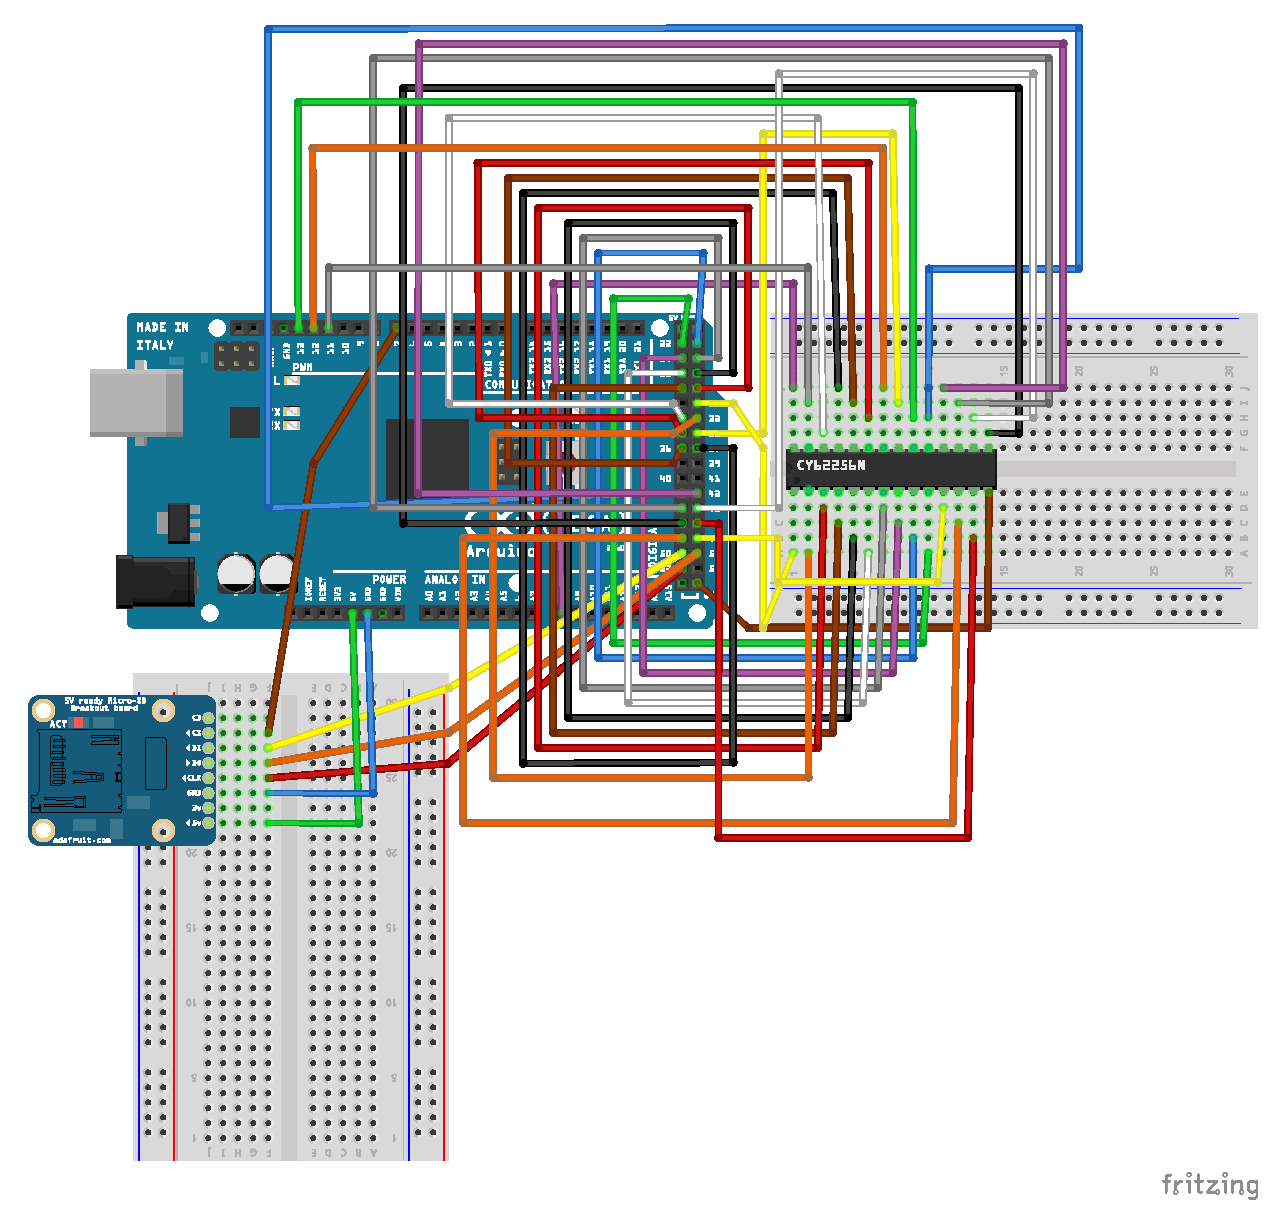
\includegraphics[width={\textwidth}]{images/CY62256-new-SD_bb}}
    \caption{An illustration on how to connect an Arduino Mega 2560 with an SRAM Cypress CY62256NLL and a micro SD.}
    \label{fig:cy62256nll_scheme_sd}
\end{figure}

% How to develop an open source secure data protection and key storage scheme using off-the-shelf SRAM component and software-based SRAM PUF technology?

\section{Procedure on Developing SRAM PUF-Based Applications Using Any Off-The-Shelf SRAM}\label{ch:procedure_develop}
After presenting the complete enrollment scheme, we also come up with a procedure to develop SRAM PUF-based applications using any off-the-shelf SRAM.
Similar to the complete enrollment scheme, this procedure scheme also consists of a PC, acting as a master, and an Arduino connected to an external SRAM component which acts as a slave. The PC side will run Python code. To reconstruct the PUF-generated key, similar to the enrollment scheme, one also only need an Arduino, no PC is needed.
This procedure will check whether the quality of off-the-shelf SRAM is sufficient as a PUF root-of-trust or not. In addition, the procedure also generates the helper data and the challenge of the SRAM which can be used to reconstruct PUF-generated key. Using this PUF-generated key, anyone can build their applications. For example, this PUF-generated key can be utilized as the root-of-trust in an authentication application. Below are the steps defined in this procedure (step 1-5 requires an Arduino and a PC, step 7 only requires an Arduino):
\begin{enumerate}
  \item Get any off-the-shelf SRAM from the market.
  \item Ensure that the Arduino and the PC are able to communicate perfectly with the off-the-shelf SRAM.
  \item Locate the stable bits using data remanence algorithm.
  \item Test the stable bits on various conditions. If the stable bits show an acceptable result, continue using this SRAM (continue to next step). Otherwise, abandon and try another off-the-shelf SRAM (go back to step 1).
  \item Generate the challenge and the helper data using the enrollment scheme shown in Section \ref{ch:complete_enrollment_scheme}. Both the helper data and the challenge is unique to the tested SRAM component.
  \item Using the challenge and the helper data, one will be able to reconstruct the PUF-generated key. Afterward, the PUF-generated key can be applied as a root-of-trust in any application.
\end{enumerate}

\section{Testing on Secure Data Protection and Key Storage Scheme}\label{ch:testing_scheme}
To check the validity of the proposed data protection and key storage scheme, several testings are performed. First, the final key generated using HMAC SHA3 is checked. Afterwards, the result of the encryption and decryption using the final key is also tested. Last, the time required in the scheme is also measured. During the time measurement, the stage is divided into multiple stages to ease the analysis.

To check the validity of the final key, a comparison between the generated final key and an online HMAC SHA3 calculator \cite{hmac_calculator} is performed. As a reminder, the key for HMAC function is the PUF generated key and the message input for the HMAC is the user's password. Below is the testing result:
\begin{itemize}
  \item PUF generated key: \seqsplit{d20f5656bf436516cd0f3d2e734851dc537df51897484128ccae67ee1310f69b}
  \begin{itemize}
    \item user's password: 70617373776f7264\newline
    final key: \seqsplit{084536fcb3135af89e1e32d423156511f13e52246acaa591b1d4115666727814}\newline
    valid: yes
    \item user's password: 6b6f6e746f6c6b61626568\newline
    final key: \seqsplit{1d1e467224d72c81ede61fcd5d1ac10535f3ebafa6e9f0d5086e6086a30787c7}\newline
    valid: yes
    \item user's password: \seqsplit{71776572747975696f706173646667686a6b6c7a786376626e6d}\newline
    final key: \seqsplit{dda21605fc56b55659cffdf57f5453a9e380aa7bd78fe52b7dc64ff4515ff4a0}\newline
    valid: yes
  \end{itemize}
  \item PUF generated key: \seqsplit{35e2f312bd28a36a359eb1a1e37f212d17da41a5b17cb2c642f5fd8e42bbd4f0}
  \begin{itemize}
    \item user's password: 70617373776f7264\newline
    final key: \seqsplit{c2892f1b1d52d59549591d410a40527b265b91d444d2032f28ce7374f7246152}\newline
    valid: yes
    \item user's password: 6b6f6e746f6c6b61626568\newline
    final key: \seqsplit{ec85915ae65f3e5141128a520327c4d5cd3119cb6769fddd948d3061dfb6fed9}\newline
    valid: yes
    \item user's password: \seqsplit{71776572747975696f706173646667686a6b6c7a786376626e6d}\newline
    final key: \seqsplit{da9e28f76754dcd4946c1343a3dd8550338d98e46d3a11e09f903204044ac9c7}\newline
    valid: yes
  \end{itemize}
\end{itemize}

After checking the validity of the final key, a testing on encryption and decryption using the final key is performed. The input data on this testing is user’s key. To check the validity of the ciphertext, an online encryption calculator \cite{aes_calculator} is utilized. The ciphertext result of the encryption process will be used as the input for the decryption test. If the decryption result is similar with the user’s key, then both encryption and decryption process in this scheme is valid.

\begin{itemize}
  \item user's key: 6a656d6275746a656d62756a656d6275
  \begin{itemize}
    \item final key: \seqsplit{084536fcb3135af89e1e32d423156511f13e52246acaa591b1d4115666727814}\newline
    ciphertext: 874cd8b8010f29f0a52eb564f1306119\newline
    ciphertext validity: yes\newline
    decryption result: 6a656d6275746a656d62756a656d6275\newline
    decryption validity: yes
    \item final key: \seqsplit{1d1e467224d72c81ede61fcd5d1ac10535f3ebafa6e9f0d5086e6086a30787c7}\newline
    ciphertext: c258a267ea58d04e0795e661000b9e4f\newline
    ciphertext validity: yes\newline
    decryption result: 6a656d6275746a656d62756a656d6275\newline
    decryption validity: yes
    \item final key: \seqsplit{dda21605fc56b55659cffdf57f5453a9e380aa7bd78fe52b7dc64ff4515ff4a0}\newline
    ciphertext: 64586f93c32e0498a46e906dc85b726a\newline
    ciphertext validity: yes\newline
    decryption result: 6a656d6275746a656d62756a656d6275\newline
    decryption validity: yes
    \item final key: \seqsplit{c2892f1b1d52d59549591d410a40527b265b91d444d2032f28ce7374f7246152}\newline
    ciphertext: f7a0c1bfdbe1d12af85ca5c3933bc29d\newline
    ciphertext validity: yes\newline
    decryption result: 6a656d6275746a656d62756a656d6275\newline
    decryption validity: yes
    \item final key: \seqsplit{ec85915ae65f3e5141128a520327c4d5cd3119cb6769fddd948d3061dfb6fed9}\newline
    ciphertext: b91b1d3031b3da73a6c1afe516d85b8b\newline
    ciphertext validity: yes\newline
    decryption result: 6a656d6275746a656d62756a656d6275\newline
    decryption validity: yes
    \item final key: \seqsplit{da9e28f76754dcd4946c1343a3dd8550338d98e46d3a11e09f903204044ac9c7}\newline
    ciphertext: 1f78480b2687b7b7faba210985600372\newline
    ciphertext validity: yes\newline
    decryption result: 6a656d6275746a656d62756a656d6275\newline
    decryption validity: yes
  \end{itemize}

\end{itemize}

Measurement of time required in this scheme is also done. During the measurement, the scheme is divided into eight stages. Stage one is on the initialization of the libraries required to access SRAM Cypress CY62256 and microSD. Stage two is when the challenge and the helper data are loaded from micro SD. The third one is calculated when reconstructing the PUF key. Next stage is during the derivation of the final key (derived from user's password and PUF-generated key). Stage five and stage six refers to the processes of encryption and saving ciphertext to microSD. Stage seven and stage eight refers to the procedure of reading ciphertext from microSD and the decryption process (reconstructing the bitcoin key). The measurement result can be seen on Table \ref{tab:time_scheme}. It can be seen that the longest time required is when loading the challenge and the helper data from the microSD (stage 2), followed by the initialization stage (stage 1). Due to this significant time required, a further optimization on accessing data from microSD is suggested in possible future works.

\begin{table}[htbp]
  \centering
  \caption{Time measurement of the secure data protection and key storage scheme in ms.}
    \begin{tabular}{|c|c|c|c|c|}
    \hline
    \textbf{No} & \textbf{Stage 1} & \textbf{Stage 2} & \textbf{Stage 3} & \textbf{Stage 4} \\
    \hline
    1     & 1022.66 & 2205.25 & 978.15 & 33.57 \\
    \hline
    2     & 1022.65 & 2205.24 & 974.39 & 33.57 \\
    \hline
    3     & 1022.63 & 2205.25 & 981.27 & 33.57 \\
    \hline
    Average & 1022.65 & 2205.25 & 977.94 & 33.57 \\
    \hline
    \textbf{No} & \textbf{Stage 5} & \textbf{Stage 6} & \textbf{Stage 7} & \textbf{Stage 8} \\
    \hline
    1     & 0.84  & 39.96 & 13.02 & 1.72 \\
    \hline
    2     & 0.85  & 39.88 & 13.02 & 1.71 \\
    \hline
    3     & 0.84  & 39.78 & 13.01 & 1.72 \\
    \hline
    Average & 0.84  & 39.87 & 13.02 & 1.71 \\
    \hline
    \end{tabular}%
  \label{tab:time_scheme}%
\end{table}%

To ensure the functionality of the system, we also constructed test cases for the source code. The testing is done only on the functionality of the system, not on the code which has a direct interaction with hardware (e.g. code to read microSD and SRAM). This decision is taken because to ensure the code is properly working, the hardware has to be in a proper condition, while checking the hardware condition is sometimes problematic and cannot be automated. The quality of the test cases is shown by code coverage which generated using GCOV and LCOV. Figure \ref{fig:code_coverage} shows the code coverage result. As seen there, there are directories where the line coverage is not 100\% covered. The reasons are some directories are just library to enable code testing (folder 'gmock' and folder 'gtest', both are libraries created by Google which required to enable the testing) and one directory is a part of LLVM compiler infrastructure (folder 'v1'). Another directory which is not fully covered is 'Crypto', this folder is a library required to do the encryption, decryption, and HMAC but provides more functional than what we need to construct the system. Thus, the test is only done on the functionality that is actually needed by the system which leads to a not full percentage of code coverage.

\begin{figure}[tph!]
    \centerline{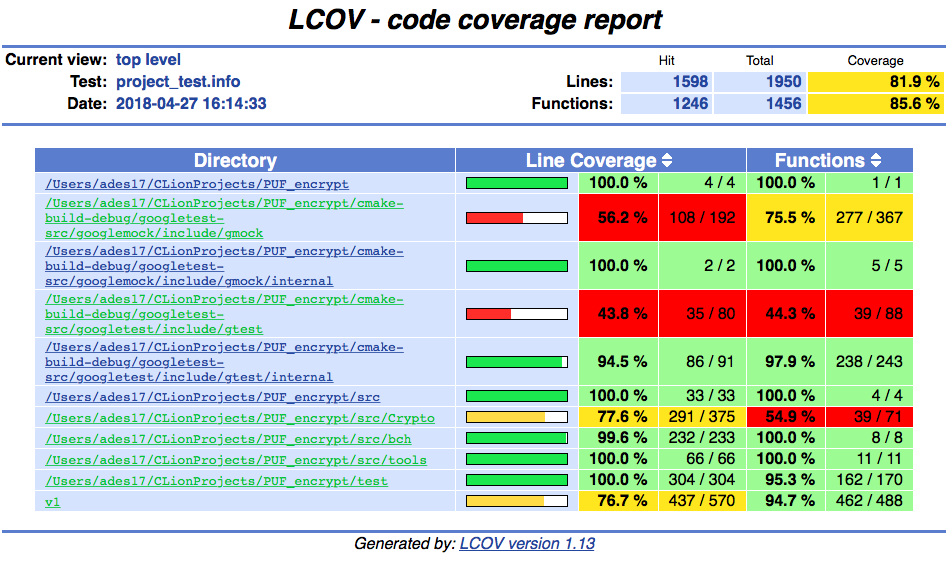
\includegraphics[width={\textwidth}]{images/code_coverage}}
    \caption{Code coverage of the constructed project.}
    \label{fig:code_coverage}
\end{figure}

% \section{Concluding Experiment with Cybercurrency}
\section{Concluding Experiment with Cybercurrency}
As the final experiment of this thesis, we present a demo of storing a private key of a cybercurrency. We believes this proves the usefulness and viability of this work for realistic use-cases. The chosen cybercurrency in this demo is Bitcoin. In Bitcoin, the private key has a length of 256-bit or 32 bytes \cite{bitcoin_key}. The experiments starts by performing an enrollment on an Arduino board with an SRAM Cypress CY62256NLL and a microSD connected to it, resulting in challenge and helper data which store in the microSD. Using the produced challenge and helper data, user creates a final key which derived from the PUF-generated key and user's password. The final key is utilized to encrypt a bitcoin key, then the ciphertext is stored in microSD. Afterwards, the Arduino is turned off.
Later, the microSD and the SRAM are transferred to another Arduino board. The new Arduino board is powered on, then it is used to reconstruct the final key by inputing the correct user's password. Finally, the reconstructed final key is applied to the ciphertext which is loaded from the microSD. The bitcoin key storing experiment is considered successful if the result of decryption is the same as the bitcoin key.
Moreover, we also shows that the bitcoin key will not be reconstructed successfully if user's password is incorrect or the SRAM is not similar with the one that use to encrypt the bitcoin key.

This experiment was done on five SRAMs Cypress CY62256NLL which can be identified by having index 'A', 'B', 'C', 'D', and E.
The result of this experiment is shown on Appendix \ref{app:screenshot}. These figures show that the stored / secured bitcoin key can only be reconstructed using a correct user's password and the exact SRAM that used during the storing (encryption) stage. If the SRAM is not similar with the one used for the encryption stage or the input password is inaccurate, the bitcoin key cannot be reconstructed to the actual one.
Based on these result, we believe that the constructed data protection and key storage scheme is secure and successfully built.

\section{Conclusion}
In this chapter, we provide explanations of several experiment setups and results. We start by presenting two chosen SRAMs that used in experiments; Microchip 23LC1024 and Cypress CY62256NLL. Both are tested on the effect of voltage variations regarding the HD\textsubscript{intra}, HD\textsubscript{inter}, distribution of 1's and 0's. Afterwards, the testing results on two bit selection algorithms (neighbor analysis and data remanence approach) and the reliability of the stable bits produced by these algorithms are displayed. From these experiments, we concluded that the Microchip 23LC1024 is unreliable to be a PUF candidate while Cypress CY62256NLL has a solid ground to be the root-of-trust of a PUF. We also able to determine that data remanence approach can produce more stable bits compared to neighbor analysis.
The chapter continues with examination on our proposed PUF challenge. Since Cypress CY62256NLL has a capacity of 262144 bits and the required bits for PUF generation is 2331 bits, there are $P(262144, 2331)=\frac{262144!}{\left( 262144-2331 \right) !}\approx 10^{12626}$ possible challenges. We also display our complete enrollment scheme and the procedure on developing SRAM PUF-based applications using any off-the-shelf SRAM. Next, testing on the designed secure data protection and key storage scheme is shown. Last, experiment outcomes on storing bitcoin private key conclude this chapter.
